%!TEX TS-program = xelatex
%!TEX encoding = UTF-8 Unicode

\documentclass{Dissertate}

\makeglossaries
\setabbreviationstyle[acronym]{long-short}

\newglossarystyle{abbrv}{
  \setglossarystyle{long}% base a 2 colonne (longtable)
  \renewcommand*{\glsgroupskip}{}% niente separatori di lettera
  \renewcommand*{\glossentry}[2]{%
    \glsentryitem{##1}%
    \textbf{\textsc{\glsentryshort{##1}}} & % colonna sinistra
    \glossentrydesc{##1}\\               % colonna destra
  }%
}

\newacronym{llm}{LLM}{Large Language Model}
\newacronym{mcp}{MCP}{Model Context Protocol}

\newacronym{jni}{JNI}{Java Native Interface}
\newacronym{ndk}{NDK}{Native Development Kit}
\newacronym{abi}{ABI}{Application Binary Interface}
\newacronym{art}{ART}{Android Runtime}
\newacronym{apk}{APK}{Android Package}
\newacronym{dex}{DEX}{Dalvik Executable}
\newacronym{aosp}{AOSP}{Android Open Source Project}
\newacronym{nnapi}{NNAPI}{Android Neural Networks }

\newacronym{cve}{CVE}{Common Vulnerabilities and Exposures}
\newacronym{cwe}{CWE}{Common Weakness Enumeration}
\newacronym{cvss}{CVSS}{Common Vulnerability Scoring System}

\newacronym{asan}{ASan}{AddressSanitizer}
\newacronym{hwasan}{HWASan}{Hardware-assisted AddressSanitizer}
\newacronym{aflpp}{AFL++}{American Fuzzy Lop++}
\newacronym{libfuzzer}{libFuzzer}{LLVM In-Process Coverage-Guided Fuzzer}

\newacronym{jit}{JIT}{Just-In-Time}
\newacronym{aot}{AOT}{Ahead-Of-Time}

\begin{document}

    % the front matter
    %!TEX root = ../dissertation.tex
\title{LLM-Based Triaging of Vulnerabilities in Android Native Libraries}
\author{Nicola Busato}
\studentId{2119291}

% If you have one advisor
\advisor{Prof. Eleonora Losiouk}

% If you are coadvised
\coadvisorOne{PhD Samuele Doria}
%\coadvisorTwo{}
\coadvisorsUniversity{University of Padova}

\university{University of Padova}
\department{Mathematics ``Tullio Levi-Civita''}
\mastername{Cybersecurity}
\academicYear{2024-2025}

    \frontmatter
    \setstretch{\dnormalspacing}
    
    % chapters
    \setcounter{chapter}{0}
    %!TEX root = ../dissertation.tex

\chapter{Introduction}
\label{chp:intro}

Android powers most of the world's smartphones (with around a 75\% market share), shaping a vast, heterogeneous ecosystem of devices, vendors, and software variants \cite{statcounter-android-2025,acar-sp16}. 

At this scale, with a marketplace hosting millions of apps and extensive reuse of the same third-party libraries across thousands of packages.%, the central security challenge is one of quantity. 
A single vulnerable native component can propagate widely.

Despite Android’s multi-layered security model, which includes application sandboxing, permission mediation, SEAndroid/SELinux policy, and verified boot, vulnerabilities persist across apps, frameworks, and vendor components \cite{acar-sp16,mayrhofer-apsm-2023}. High-impact examples include memory-safety vulnerabilities in media codecs, that have enabled fully remote, zero-interaction compromise of commercial devices delivered via MMS \cite{p0-qmage}. 
Furthermore, empirical evidence indicates that popular apps often embed third-party components with known \glsxtrshortpl{cve} and that patch adoption on the app side often lags behind fixes to upstream libraries \cite{almanee-icse21}.

Within this landscape, many Android applications embed native C/C++ libraries to achieve low latency, reuse existing code, or access device- and vendor-specific functionality. These libraries are invoked across the \glsxtrshort{jni} boundary, which bridges managed code and native components. While effective for performance, this practice imports the memory-unsafe semantics of C/C++ into an otherwise memory-safe application model, increasing the likelihood of buffer overflows, use-after-free, and related memory-corruption defects. Because native code executes in the same process as the \glsxtrshort{art}, a flaw in the native layer can compromise the entire app and its data, irrespective of the safety of its Java/Kotlin components \cite{almanee-icse21, mergendahl-ndss22}.

\textcolor{blue}{"non puoi introdurre il fuzzing così velocemente. Passi dal discorso generale di vulnerabilità lato nativo e poi, diretto, all'uso di fuzzing"}

\textcolor{red}{A common approach to uncover software defects at scale is fuzzing, an automated dynamic testing technique that feeds programs with large volumes of unexpected, invalid, or mutated inputs to trigger abnormal behaviours. By exercising a wide range of execution paths, fuzzing reveals crashes that may indicate underlying vulnerabilities.}

Recent works automate the generation of harnesses and large-scale fuzzing for Android native libraries. Tools such as POIROT can synthesise app-specific harnesses that support bidirectional \glsxtrshort{jni} interactions and then fuzz them at scale, reporting thousands of distinct crashes and confirmed vulnerabilities \cite{poirot-usenix25}. 
However, triaging the resulting crashes, separating benign faults from security-relevant memory errors, remains largely manual.

%; existing bucketing and “exploitability” heuristics have limited precision and still require substantial analyst oversight \cite{}.

This thesis investigates whether a tool-grounded \gls{llm} can reduce manual effort and improve consistency in crash triage for Android native libraries. To this end, it introduces an architecture\footnote{Implementation available at \url{https://github.com/Nicola-01/LLM-Triaging}.} in which POIROT causes crashes; an \gls{llm}-based triager consumes the associated reports and augments them with program context via the \gls{mcp}, invoking reverse-engineering tools (Jadx for Dalvik/bytecode and manifest, and Ghidra for native disassembly/decompilation) to recover stack evidence, function names, and short decompiled snippets.
The triager classifies whether a crash likely indicates a vulnerability, explains the rationale in plain terms, provides a severity estimate anchored to standard taxonomies/scores (\glsxtrshort{cwe}/\glsxtrshort{cvss}), and suggests follow-up actions. % (\gls{cwe}/\gls{cve}/\gls{cvss}) % forse no cve
    \chapter{Background}
\label{chp:backgroud}

\section{Android Native}
Android itself relies extensively on native C/C++ libraries within its core architecture. Many system components and services, such as the runtime, media stack, graphics pipeline, and hardware abstraction layer (HAL), are implemented in native code for reasons of performance, portability, and direct hardware access \cite{android-platform}. The framework exposes parts of this functionality to applications through Java/Kotlin \glspl{api}, enabling managed code to invoke native system services when needed. 

At the system level, Android’s C standard library and dynamic linker are provided by \emph{Bionic}, a lightweight libc/libm/libdl implementation optimised for mobile environments \cite{bionic-maint}. This design allows the platform to combine managed execution (via the \gls{art}) with efficient, low-level components responsible for performance-critical and hardware-dependent operations. Figure~\ref{fig:androidStack} illustrates the Android platform architecture, highlighting how native libraries underpin the runtime, system services, and the HAL.

Beyond the platform itself, developers can extend Android apps with their own native code through the \gls{ndk}.

The advantages of native development stem from the ability to execute compiled machine code directly on the target CPU, allowing finer-grained optimisation and efficient memory use, important for resource-constrained mobile devices. It also enables hardware acceleration and access to specialised \glspl{api} (e.g., GPU, DSP, or sensor interfaces), making it indispensable in areas like augmented or virtual reality, game engines (e.g., Unity, Unreal), and device-specific system utilities.% \textcolor{red}{Dovrei cercare una citazione}

However, using native code extends the scope of Android applications beyond the safety of the managed runtime. Developers must explicitly handle memory allocation and deallocation, thread synchronisation, and exception propagation, as these are not automatically managed by the \gls{art}. Cross-ABI compatibility, debugging complexity, and maintenance across Android versions further increase the development load. Consequently, the \gls{ndk} is recommended only when its benefits outweigh these costs \cite{android-ndk-getting-started,android-ndk-concepts,jni-tips}.

This capability to use native code extends the reach of Android apps beyond the managed runtime but also introduces explicit responsibilities for developers. Native code must handle its own memory management, threading and exception handling. This is significantly different from pure Java/Kotlin development.

\begin{figure}
    \centering
    \begin{tikzpicture}

    \tikzset{
        groupbox/.style={inner sep=0pt}
    }

    \def\W{8cm}
    \def\Wleft{4.45cm}
    \def\Wright{3.45cm}
    \def\Distance{0.8mm}
    
    \node[layer, fill=cSystem!60, minimum width=\W] (apps) {System Apps};
    \node[layer, fill=cJava!60, minimum width=\W, below=\Distance of apps] (java) {Java API Framework};
    
    \node[layer, fill=cNative!60, minimum width=\Wleft, below=\Distance of java, anchor=west] (native) at ($(java.south west)+(0,-3.5mm)$) {Native C/C++ Libraries};
    \node[layer, fill=cRuntime!70, minimum width=\Wright, below=\Distance of java, anchor=east] (runtime) at ($(java.south east)+(0,-3.5mm)$) {Android Runtime};
    
    \node[groupbox, fit=(native) (runtime)] (BOX) {};
    
    \node[layer, fill=cHAL!60, minimum width=\W, below=\Distance of BOX] (hal) {Hardware Abstraction Layer (HAL)};
    \node[layer, fill=cKernel!60, minimum width=\W, below=\Distance of hal] (kernel) {Linux Kernel};
\end{tikzpicture}

    \caption[Android software stack.]%
    {Android software stack \cite{android-platform}}
    \label{fig:androidStack}
\end{figure}

\subsection{\glsxtrlong{ndk}}
The \gls{ndk} is a collection of tools, headers, and libraries that enable developers to embed C and C++ code within Android applications and interact natively with hardware, sensors, and system \glspl{api} \cite{android-ndk-getting-started}. The \gls{ndk} supports compilation into shared (and static) libraries that can be packaged inside the \gls{apk}, and offers native interfaces for tasks such as sensor input, asset loading, and more \cite{android-ndk-concepts}.

Developers typically adopt native code for three main reasons:
\begin{itemize}
  \item \textbf{Performance optimization:} achieving low-latency processing in compute-intensive domains such as graphics, signal processing, physics, or cryptography.
  \item \textbf{Library reuse:} integrating existing C/C++ libraries (e.g.\ cryptography, compression, codecs) to avoid rewriting functionality in Java/Kotlin.
  \item \textbf{Hardware or vendor-specific access:} interacting directly with low-level or proprietary \glspl{api} (e.g.\ custom sensors, specialized accelerators) not exposed in the Java framework.
\end{itemize}

However, using the \gls{ndk} comes with tradeoffs. Native development adds complexity in build configuration, cross-ABI support, debugging, and maintenance across Android versions. Not all Android \glspl{api} are directly available through the \gls{ndk}, so bridging via \gls{jni} is often required for broad framework functionality \cite{android-ndk-concepts}. 

\subsection{\glsxtrlong{jni}}
The \gls{jni} (Java Native Interface) is a native programming interface that enables Java or Kotlin code running in a virtual machine to interoperate with libraries and applications written in C/C++ \cite{jni-spec-intro}. It allows managed code to call into native code, and for native code to call back into the \gls{vm}, manipulate Java objects, throw exceptions, and more. The \gls{jni} is designed to impose no restrictions on the implementation of the \gls{vm}, thereby preserving binary compatibility across \gls{vm} vendors \cite{jni-spec-intro}.  

Listing~\ref{lst:javaNative} shows a Java class declaring a \texttt{native} method, while Listing~\ref{lst:JNI} gives the corresponding C implementation on the native side.

\begin{lstlisting}[language=Java+JNI, caption={Java class declaring a \texttt{native} method}, label={lst:javaNative}] 
public class foo {
    private native double bar(int i, String s);
    static {
        System.loadLibrary("native-lib");
    }
}
\end{lstlisting}

\begin{lstlisting}[language=C+JNI, caption={Native implementation of \texttt{bar}}, label={lst:JNI}]
jdouble Java_pkg_foo_bar(JNIEnv *env,          // ptr to JNI interface
                         jobject obj,          // "this" pointer
                         jint i, jstring s) {  // first and second parameter
    return 0.0; /* Method implementation */
}
\end{lstlisting}


\begin{comment}
    \subsection{Vulnerabilities} %  and Impact on the Android Sandbox
Bugs in native memory safety remain the main cause of serious compromise on Android. 
Although the platform’s sandbox assigns each app a distinct \gls{uid} and constrains it further with SELinux policies, a native component compromised inside that boundary still runs with the app’s privileges and can expose any secrets or capabilities already permitted (e.g., tokens, stored content, or keys) \cite{android-app-sandbox,android-selinux}. In practice, this turns local corruption into high-impact data access or control-flow hijacking even without crossing process boundaries.
Memory-safety defects in native libraries, such as buffer overflows, out-of-bounds reads/writes, use-after-free, and double free, belong to well-known categories captured by \gls{cwe}, and they frequently appear in \gls{cve} records \cite{cwe-mitre,cve-overview}. On Android, these errors may manifest as application crashes, or in more severe cases permit arbitrary code execution or data tampering, depending on mitigations and exploitability assumptions \cite{android-native-risk}. 


Attackers often amplify impact by chaining flaws across interfaces. Many system services are native and reachable over Binder; memory corruption in such a service can be triggered via \gls{ipc} by a malicious client to escape app-level limits \cite{mao-nass-usenix25}. 

In other scenarios, native code may corrupt memory pages shared with the managed runtime (e.g. altering \gls{jni} or class metadata) by transgressing memory protection via system calls (e.g. \texttt{mprotect}), thus undermining Java-level safety invariants and enabling code injection or VM subversion \cite{going-native-ndss17}. 
Another common vector is outdated third-party native libraries: empirical studies show that a significant fraction of popular apps ship unpatched vulnerable native libraries, and that developers take on average hundreds of days to apply upstream patches \cite{almanee-icse21}. This “patch latency” enables attackers to exploit known vulnerabilities even in apps that seem benign at the Java layer.  

Mitigation requires defense-in-depth: modern Android hardening (ASLR/DEP, control-flow integrity, memory tagging), combined with strict interface design and timely library updates, can substantially raise exploitation cost even when bugs persist \cite{android-ndk-mte}. 
\end{comment}

\subsection{Vulnerabilities and Impact on the Android Sandbox}
Native memory-safety bugs remain a dominant cause of serious compromise on Android. Although the platform’s sandbox assigns each app a distinct \gls{uid} and further constrains it with SELinux policies, a native component compromised inside that boundary still runs with the app’s privileges and can expose secrets or capabilities already permitted (e.g., tokens, stored content, keys) \cite{android-app-sandbox,android-selinux}. In practice, this turns local corruption into high-impact data access or control-flow hijacking even without crossing process boundaries.

Memory-safety defects in native libraries, such as buffer overflows, out-of-bounds reads/writes, use-after-free, and double free, belong to well-known \gls{cwe} families and frequently appear in \gls{cve} records. %\cite{cwe-mitre,cve-overview} 
On Android, these errors may cause crashes or, in more severe cases, permit code execution or data tampering depending on mitigations and exploitability assumptions \cite{android-native-risk}.

Attackers often amplify impact by chaining flaws across interfaces. Many system services are native and reachable over Binder; memory corruption in such a service can be triggered via \gls{ipc} by a malicious client to bypass app-level limits \cite{mao-nass-usenix25}. In other scenarios, native code may corrupt memory shared with the managed runtime (e.g., altering \gls{jni} or class metadata) by abusing memory-protection system calls, undermining Java-level safety invariants and enabling code injection or \gls{vm} subversion \cite{going-native-ndss17}. Another common vector is outdated third-party native libraries: empirical studies show that a significant fraction of popular apps ship unpatched vulnerable native libraries, and that developers take on average hundreds of days to apply upstream patches \cite{almanee-icse21}. This patch latency enables exploitation of known bugs even in apps that appear benign at the Java layer.

% Mitigation requires defense-in-depth: modern Android hardening (\gls{aslr}/\gls{dep}, control-flow integrity, memory tagging), combined with strict interface design and timely library updates, can significantly reduce the feasibility and reliability of exploitation even when bugs persist \cite{android-ndk-mte}.

\section{Fuzzing}
Fuzzing is an automated testing technique that repeatedly executes a target program with many inputs, either randomly generated or systematically derived, to expose defects such as crashes, assertion failures, or memory-safety violations. Modern fuzzers prioritise inputs that increase code coverage (e.g., edge or block coverage), and couple execution with hardening oracles (e.g., sanitizers) to turn latent memory errors into reliable, actionable signals \cite{sutton2007fuzzing,godefroid2008sage}.

\subsection{Types}
A fuzzer can be classified along three ways:
\begin{itemize}
  \item \textbf{Input production:} \emph{generation-based} where inputs are produced from a model or specification and \emph{mutation-based} where inputs are produced by mutating existing seeds. Coverage-guided mutation fuzzers (e.g., AFL++, libfuzzer) iteratively mutate seeds that increase coverage.
  \item \textbf{Input knowledge:} \emph{structured}, grammar- or model-based, aware of input format/protocol, or \emph{unstructured}, no knowledge of structure; “dumb” or purely random.
  \item \textbf{Program knowledge:} \emph{black-box}: no visibility into internals, \emph{grey-box}: lightweight instrumentation, e.g., edge coverage, and \emph{white-box}: constraint solving/symbolic execution to systematically steer execution, as in SAGE \cite{godefroid2008sage}.
\end{itemize}

\subsection{Uses}
Fuzzing is primarily employed to discover security-relevant defects in safety- or security-critical software. Its strength lies in \emph{demonstrating the presence} of bugs via concrete, reproducible inputs. Proving correctness for all inputs requires a formal specification and formal methods; fuzzing complements, rather than replaces, such approaches \cite{sutton2007fuzzing}. In practice, fuzzing integrates into secure development lifecycles and Continuous Integration pipelines to continuously test libraries, parsers, and interfaces that process untrusted data.

\subsection{Android context} %  (sanitizers as oracles).
On Android, fuzzing native components benefits from memory error detectors such as Hardware-assisted AddressSanitizer (HWASan) and, historically, AddressSanitizer (ASan). These sanitizers instrument code to detect out-of-bounds accesses, use-after-free, and related violations during fuzzing, producing precise diagnostics that accelerate crash triage \cite{hwasan-ndk,asan-aosp,asan-clang}.

Two widely used coverage-guided engines are American Fuzzy Lop++ (AFL++) (a fork and extension of AFL with a rich ecosystem of mutators and instrumentation options) and LLVM In-Process Coverage-Guided Fuzzer (libFuzzer). Both have been successfully applied to native libraries, including on Android, to elicit high-quality crashes and to maximise coverage under realistic budgets \cite{aflpp-woot20,libfuzzer-llvm}.






\section{\glsxtrlong{llm}}
\glspl{llm} are deep neural networks based on the Transformer architecture, which replaces recurrence/convolution with stacked self-attention and feed-forward layers to model long-range dependencies efficiently \cite{vaswani2017attention}. Today’s \glspl{llm} are pre-trained on large corpora via next-token prediction and then adapted to follow user prompts. 

\subsection{Limitations and Hallucinations}
Because \glspl{llm} predict tokens rather than verify facts, they can generate confident but incorrect content (``hallucinations''). Surveys and recent studies document multiple forms (e.g., intrinsic or confabulated outputs) and show that even state-of-the-art models may produce fluent fabrications \cite{ji2023hallucination,farquhar2024semanticentropy}. In security-oriented workflows such as vulnerability triage, this can manifest as invented \gls{cve} identifiers, non-existent \glspl{api} or packages, fabricated proof-of-concept details, or misattributed stack traces, errors that can mislead severity assessment or waste analyst time. Empirical work on code-generation further highlights ``package hallucinations'', where models recommend non-existent libraries, creating supply-chain risk if an attacker later publishes a malicious package with that name \cite{spracklen2025package}. 
%Consequently, any use of \glspl{llm} for triage should treat outputs as hypotheses to be checked against authoritative sources and artefacts (code, binaries, advisories), and prefer designs that promote verifiability and uncertainty signalling rather than unconditional trust.



\section{\glsxtrlong{mcp}}
\gls{mcp} is an open protocol, introduced by Anthropic (creator of Claude) in November 2024, that standardises how \gls{ai} applications obtain and manage external context via a client–server architecture.
An \emph{MCP host} (the \gls{ai} application) connects to one or more \emph{MCP servers} through dedicated \emph{MCP clients}, enabling the host to discover and use tools, read resources, and apply prompts exposed by servers. The protocol separates \emph{data layer} (primitives, lifecycle, notifications) from a \emph{transport layer} (e.g., stdio for local, streamable HTTP for remote), so the same message semantics work across local and remote deployments \cite{mcp-architecture,mcp-intro, mcp-transports}. In brief, servers contribute context and actions; clients manage capability negotiation and exchanges; the host orchestrates everything in the user-facing application \cite{mcp-architecture,mcp-server-concepts,mcp-client-concepts}. Figure~\ref{fig:mcp-simple-diagram} provides a high-level view of this host–client–server pattern and example integrations.

\begin{figure}
    \centering
    \scalebox{0.8}{\begin{tikzpicture}[font=\small, node distance=5mm and 16mm]

% --- Stili per i box principali ---
\tikzset{
  groupbox/.style={inner sep=0pt},
  grouplabel/.style={font=\footnotesize\bfseries, fill=white, inner sep=1pt}
}

\def\WNode{45mm}
\def\HNode{25mm}
\def\NDistanceH{10mm}
\def\NDistanceV{2mm}

% =============== BLOCCO SINISTRA (SX): 3 elementi ===============
\node[layer, minimum width=\WNode] (L1) {\textbf{Chat interface}\\Claude Desktop};
\node[layer, minimum width=\WNode, below=\NDistanceV of L1] (L2) {\textbf{IDEs and code editors}\\Claude Code, Goose};
\node[layer, minimum width=\WNode, below=\NDistanceV of L2] (L3) {\textbf{Other AI applications}\\5ire, Superinterface};
% Box che "abbraccia" i tre nodi: il suo centro è a metà verticale
\node[groupbox, fit=(L1) (L3), label={[grouplabel, label distance=\NDistanceV]south:\gls{mcp} Hosts}] (SXBOX) {};

% =============== BLOCCO CENTRALE (CENTRO): 1 elemento ===========
% Posizionato "right=..." RISPETTO A SXBOX (non L1): così condivide la stessa y del centro
\node[layer, fill=cHAL!60, minimum width=\WNode, minimum height=\HNode, right=\NDistanceH of SXBOX] (C1)
  {\textbf{MCP}\\Standardized protocol};
\node[groupbox, fit=(C1)] (CTBOX) {};

% =============== BLOCCO DESTRA (DX): 3 elementi =================
% Posiziona il blocco destro a destra del nodo centrale (che è ora centrato verticalmente)
\node[layer, minimum width=\WNode, right={\NDistanceH*2+\WNode} of L1] (R1) {\textbf{Data and file systems}\\PostgreSQL, SQLite, GDrive};
\node[layer, minimum width=\WNode, below=\NDistanceV of R1] (R2) {\textbf{Development tools}\\Git, Sentry, etc.};
\node[layer, minimum width=\WNode, below=\NDistanceV of R2] (R3) {\textbf{Productivity tools}\\Slack, Google Maps, etc.};
\node[groupbox, fit=(R1) (R3), label={[grouplabel, label distance=\NDistanceV]south:\gls{mcp} Server}] (DXBOX) {};

% --- Stile frecce ---
\tikzset{
  bidi/.style={
    draw=black!35,
    line width=0.5pt,
    rounded corners=2mm,
    {Latex[length=2mm]}-{Latex[length=2mm]}
  },
}


\def\ADistanceH{\NDistanceH*0.5}
\def\ADistanceV{6mm}

\draw[bidi] (L1.east) -|  ([shift=({-\ADistanceH, \ADistanceV})]C1.west) -- ([yshift={\ADistanceV}]C1.west);
\draw[bidi] (L2.east) -- (C1.west);
\draw[bidi] (L3.east) -|  ([shift=({-\ADistanceH, -\ADistanceV})]C1.west) -- ([yshift={-\ADistanceV}]C1.west);


\draw[bidi] ([yshift={\ADistanceV}]C1.east) --  ([shift=({\ADistanceH, \ADistanceV})]C1.east) |- (R1.west);
\draw[bidi] (C1.east) -- (R2.west);
\draw[bidi] ([yshift={-\ADistanceV}]C1.east) --  ([shift=({\ADistanceH, -\ADistanceV})]C1.east) |- (R3.west);




\end{tikzpicture}
}
    \caption[High-level MCP architecture.]%
      {High-level \gls{mcp} architecture. The \gls{mcp} host (e.g., chat interface or IDE) coordinates one or more \gls{mcp} clients, each connected to an \gls{mcp} server that exposes tools, resources, and prompts \cite{mcp-intro}.}
    \label{fig:mcp-simple-diagram}
\end{figure}

\subsection{MCP Host}
The \gls{mcp} \emph{host} is the application the user directly interacts with (e.g., a chat UI or an IDE extension). It manages the overall user experience, session lifecycle, permissions, and tool exposure, and it instantiates one or more \gls{mcp} clients to talk to specific servers. In practice, the host governs policy (e.g., which servers are allowed, rate limits) and mediates the user-facing rendering of server responses \cite{mcp-architecture}. 
Figure~\ref{fig:mcp-interaction} situates the host on the left, coordinating multiple client–server links while preserving a single conversational surface for the user.

\subsection{MCP Client}
An \gls{mcp} \emph{client} is a protocol-level component created by the host to communicate with exactly one \gls{mcp} \emph{server}. Each client maintains a transport (stdio or HTTP/WS), negotiates capabilities, and exposes the server’s tools/resources/prompts to the host. This indirection lets the host manage several servers in parallel without coupling UI logic to any server implementation details \cite{mcp-client-concepts}. 
In Figure~\ref{fig:mcp-interaction}, clients appear as the ''middle`` connectors: they translate host intents (e.g., ''run tool T``) into \gls{api} call and relay the server’s results back to the host.

\subsection{MCP Server}
An \gls{mcp} \emph{server} wraps external systems (e.g. files, databases, reverse-engineering tools) and presents them as protocol objects: tools: invokable functions with JSON Schemas, resources: readable artefacts, and prompts: reusable task templates. Servers publish a capability manifest so that clients can discover what is available and how to access it. The \gls{mcp} \emph{server} provides tools that enable \glspl{llm} to perform actions, carry out deterministic computations and interact with external services. 
This design decouples model/UX from system integrations and enables reuse across different hosts and models \cite{mcp-tools}. 
In Figure~\ref{fig:mcp-interaction}, servers sit on the right, each encapsulating one integration boundary (e.g., Jadx, Ghidra, a code search index).

\begin{figure}
    \centering
    \scalebox{0.8}{  \begin{sequencediagram}
    % Participants
    \newinst[0]{U}{User}{}
    \newinst[1]{L}{LLM}{}
    \newinst[1]{C}{MCP Client}{}
    \newinst[1]{S}{MCP Server}{}

    % --- Capability discovery (top half) ---
    \begin{sdblock}{Initialization}{}
        \begin{call}{C}{List Tools Request}{S}{List of Tools}
        \end{call}
    
        \begin{mess}{C}{List of Tools}{L}
        \end{mess}
    \end{sdblock}


    % --- User interaction and tool invocation (bottom half) ---
    \begin{sdblock}{Invocation}{}
        \begin{call}{U}{User prompt}{L}{Reply to User}
            \begin{call}{L}{Tool Selection}{C}{Tool Response}
                \begin{call}{C}{Tool Call}{S}{Tool Response}
                    
                \end{call}
            \end{call}
        \end{call}
    \end{sdblock}

  \end{sequencediagram}}
    \caption[MCP interaction]{MCP interaction: capability discovery, tool selection, invocation, and reply.}
    \label{fig:mcp-interaction}
\end{figure}

\subsection{Interaction}
Figure~\ref{fig:mcp-interaction} illustrates a typical flow. 
\begin{enumerate}
  \item The host initialises and lists available servers (or lets the user attach new ones). % cf. MCP architecture
  \item For each server, the host spawns a client that performs capability discovery (tools/resources/prompts and their schemas). % discovery
  \item When the user or an agentic workflow triggers an action, the host selects an appropriate tool and routes a request through the corresponding client to the target server. % routing
  \item The server executes the tool (e.g., decompile a class with Jadx, disassemble a function with Ghidra) and returns structured results to the client. % tool exec
  \item The client relays the structured results to the host; the host provides this context to the \gls{llm}, and may chain further tool calls. % host mediation + elicitation
  \item The \gls{llm} synthesises a user-facing response using the returned context; the host renders this reply in the UI (and records any artefacts/evidence links). % <-- added item
  \item The host may persist state and expose follow-up actions (e.g., re-run with new arguments, open related resources), maintaining a single conversational surface. % follow-ups
\end{enumerate}


\section{Vulnerability Scoring Systems}
Modern vulnerability workflows rely on interoperable standards that identify issues, classify their root causes, and communicate technical severity. 

\subsection{\glsxtrlong{cwe}}
The \gls{cwe} is a community-curated taxonomy of common software and hardware weakness types (e.g., buffer overflow, use-after-free). It provides standardised identifiers and structured descriptions to support detection, prevention, and education across the secure development lifecycle \cite{cwe-about}. Unlike CVE (which tracks specific \emph{instances}), \gls{cwe} captures \emph{classes} of underlying faults, enabling aggregation and trend analysis at the root-cause level \cite{cwe-list}.

\subsection{\glsxtrlong{cve}}
The \gls{cve} Programme assigns unique identifiers to publicly disclosed vulnerabilities, providing a single canonical reference for coordination across vendors, researchers, and users. A \gls{cve} entry names the specific issue (product, version, and vulnerability description) and links to public references; other databases may enrich it with severity and technical details \cite{cve-overview}. In practice, national or vendor repositories (e.g., \gls{nvd}) attach \gls{cvss} scores and map each \gls{cve} to one or more \gls{cwe} categories for analytics and prioritisation \cite{nvd-cve-process,cvss40-nvd-support}.

\subsection{\glsxtrlong{cvss}}
The \gls{cvss} is an open, vendor-neutral framework for describing the intrinsic characteristics and severity of a vulnerability through a set of metrics that yield a numerical score and qualitative severity band. \gls{cvss} communicates \emph{severity}, not overall \emph{risk}; operational risk assessment should incorporate asset context, threat activity, and environmental factors beyond the Base score \cite{cvss31-user-guide}.

\paragraph{Relation}
In triage and remediation workflows, \gls{cve} entries identify concrete vulnerabilities; each entry can be mapped to \gls{cwe} identifiers that explain the underlying weakness type; \gls{cvss} scores (often provided by downstream databases) express the vulnerability’s technical severity. Together, \gls{cwe}$\rightarrow$\gls{cve}$\rightarrow$\gls{cvss} forms a pipeline from root-cause taxonomy to instance tracking and severity quantification \cite{nvd-cve-process}.

\section{Reverse engineering}
Reverse engineering in software is the analysis of binaries or bytecode to recover design and implementation information-disassembly, control/data flows, and higher-level structure, when source or specifications are incomplete or unavailable \cite{springer-sre-overview,samuelson1990re}. In practice, reverse engineering workflows combine a disassembler/decompiler with cross-reference search, symbol inspection, and targeted decompilation to produce evidence suitable for auditing and triage.

\subsection{Ghidra}
Ghidra is an open-source software reverse-engineering framework developed by the National Security Agency (NSA. It provides disassembly, decompilation, graphing, and scripting across multiple architectures, and is widely used in vulnerability research and malware analysis \cite{ghidra-github}. 

\subsection{Jadx}

Jadx is a decompiler providing Java source code from Android Dex and Apk files, with \gls{cli} and \gls{gui} front-ends; it is commonly used to inspect Android manifests, classes, and resources. In the pipeline, Jadx supplies managed-side context (e.g., App manifest, class/method signatures, entry points).


    \chapter{Related Work}
\label{chp:relatedWork}

\begin{comment}
    
\section{Fuzzing of Android native libraries and harness generation}
Fuzzing of Android native libraries poses challenges beyond conventional user-space fuzzing due to the \gls{jni} boundary, lifecycle constraints, and the need for realistic cross-language call sequences. POIROT automatically synthesises consumer-specific harnesses for closed-source Android libraries by analysing Java-side usage and supporting bidirectional \gls{jni} interactions, enabling large-scale campaigns that uncovered thousands of unique crashes \cite{poirot-usenix25}. Atlas similarly targets Android closed-source native libraries with a cross-language fuzzing framework and automatic harness generation \cite{atlas-issta24}. Beyond the Android setting, FuzzGen synthesises library-specific fuzzers by inferring API contracts and integrating with \gls{libfuzzer} to reach deep states \cite{fuzzgen-usenix20}. Prior engineering work shows that reproducing \gls{art} behaviour and \gls{jni} semantics is critical for validity and reproducibility of results \cite{polito-android-native-fuzzing}. As to fuzzing engines, \gls{aflpp} extends greybox fuzzing with a rich ecosystem of mutators and instrumentation \cite{aflpp-woot20}, while \gls{libfuzzer} offers tight integration with LLVM sanitizers for in-process fuzzing \cite{libfuzzer-llvm}. Sanitizers such as \gls{asan} and \gls{hwasan} are widely used to diagnose memory-safety defects during fuzzing on Android \cite{asan-android-aosp,hwasan-ndk}.

\section{Crash triage and LLM-based vulnerability classification}
Traditional crash triage combines bucketing, deduplication, and heuristic \emph{exploitability} estimation, but typically requires expert oversight and offers limited precision across diverse crash types \cite{scb-ase18,igor-ccs21}. Recent studies investigate \gls{llm}-assisted triage. CASEY reports non-trivial accuracy for CWE classification (68\%) and severity identification (73.6\%) on an NVD-derived corpus, indicating that \gls{llm}s can streamline parts of vulnerability triage \cite{casey-aic25}. LProtector explores \gls{llm}-driven vulnerability detection for C/C++ projects with retrieval augmentation, highlighting benefits and pitfalls of model-in-the-loop security analysis \cite{lprotector-2024}. Broader surveys benchmark \gls{llm}s and agents for practical software security, consolidating evidence that model judgements improve when provided with structured context and repository-level signals, but also documenting variability across tasks and datasets \cite{acl25-llm-benchmark-slr,slr-llm-vuln-2025}. These findings motivate tool-grounded designs for triage under Android/\gls{jni} constraints.

\section{Tool grounding with \gls{mcp} for program analysis and reverse engineering}
Tool grounding aims to reduce hallucinations and improve faithfulness by letting the \gls{llm} query authoritative artefacts. The \gls{mcp} standardises how models connect to external tools and data sources \cite{mcp-overview,anthropic-mcp}. In our setting, grounding uses Jadx to retrieve bytecode/manifest context and Ghidra for disassembly/decompilation. An emerging ecosystem of \gls{mcp} servers exposes reverse-engineering capabilities of Ghidra to \gls{llm}-based clients (e.g., symbol and function listings, decompilation), facilitating evidence-linked reasoning \cite{ghidra-mcp-laurie,ghidra-mcp-suid}. While promising, the security surface of tool integrations must be considered; recent supply-chain incidents around \gls{mcp} servers highlight the need for permission scoping and integrity checks \cite{mcp-supplychain-incident}. Our design leverages \gls{mcp} to fetch verifiable snippets (stack frames, function names, minimal decompiled code) that the triager references in its rationale.

\section{Positioning}
Compared to POIROT and Atlas, which focus on automating harness generation and fuzzing at scale \cite{poirot-usenix25,atlas-issta24}, our work targets the \emph{post-fuzzing} triage stage for Android native crashes. Relative to CASEY/LProtector and survey results on \gls{llm}-for-security \cite{casey-aic25,lprotector-2024,acl25-llm-benchmark-slr,slr-llm-vuln-2025}, our contribution is a tool-grounded pipeline that couples \gls{mcp}-mediated access to Jadx/Ghidra with crash artefacts from POIROT, aiming to improve precision, explainability, and analyst verification for \gls{jni}-mediated memory-safety issues.

\end{comment}

The proposed approach lies at the confluence of coverage-guided fuzzing and bottom-up harness generation, and recent applications of \gls{llm}s to vulnerability classification and triage. We organise prior work into four strands: (i) methodologies for automated vulnerability discovery via fuzzing; (ii) \gls{llm}-assisted harness generation and mitigation of false positives; (iii) \gls{llm}-based vulnerability triage and assessment; and (iv) reasoning and validation-feedback loops that improve reliability of automated analyses.

\section{Automated vulnerability detection and fuzzing}

Fuzz testing remains a principal technique for uncovering defects and security issues at scale. A useful distinction is between top-down fuzzing of public entry points and bottom-up fuzzing of internal functions, the latter demanding specialised drivers to translate unstructured inputs into well-formed, semantically valid API arguments \cite{jiang2024fuzzing}. Recent \gls{llm}-assisted fuzzing frameworks demonstrate that language models can increase input diversity and sustain long-horizon exploration, provided that prompting strategies adaptively distil documentation and examples into effective prompts and evolve them during the fuzzing loop \cite{10.1145/3597503.3639121}. However, bottom-up strategies are especially prone to invalid drivers and unrealistic executions, which in turn inflate the rate of spurious crashes.

\section{\gls{llm}-assisted harness generation and false-positive mitigation}

Two complementary directions address the fidelity of generated drivers and the veracity of reported crashes. First, \emph{knowledge-driven} harness generation uses code metadata, API documentation and usage correlations to guide \gls{llm}s; a \emph{sanitizer} module then fixes compilation/runtime issues and performs crash analysis to separate harness misuse from genuine bugs, feeding newly inferred constraints back into the knowledge base \cite{liupromefuzz}. Second, multi-agent schemes for large-scale driver generation propose (i) a Function Analyzer that extracts input/state constraints from code to proactively reduce misuse, and (ii) a Crash Validation agent that checks whether a crash is feasible from real entry points, filtering out a substantial fraction of false positives \cite{amusuo2025falsecrashreducermitigatingfalsepositive}. These works collectively indicate that constraint-aware generation and post hoc feasibility checks are both necessary to keep precision high when scaling bottom-up fuzzing.

\section{\gls{llm}-based vulnerability triage and assessment}

Beyond discovering crashes, several studies target automated triage: mapping issues to \gls{cwe} categories and estimating severity under \gls{cvss}. CASEY shows that \gls{llm}s can classify \gls{cwe} and approximate \gls{cvss} labels from structured descriptions and compact code hunks, with fine-tuning improving accuracy and stability on an NVD-derived dataset \cite{torkamani2025streamlining}. LProtector employs binary classification with Retrieval-Augmented Generation (RAG) to inject domain knowledge and reports improved F1 on Big-Vul, suggesting that retrieval helps compensate for limited in-context capacity \cite{sheng2024lprotectorllmdrivenvulnerabilitydetection}. A broader multi-task evaluation finds that while traditional transformers remain competitive for pure detection, code-centric \gls{llm}s excel at assessment/localisation when provided with key contextual artefacts (e.g., \gls{cve} descriptions, commits) \cite{10706805}. Earlier work on continuous monitoring likewise reports useful initial classification performance but highlights sensitivity to noisy descriptions and the need for stronger validation signals \cite{10456393}. Together, these results motivate a triage pipeline that privileges concise, structured context and emphasises evidence that analysts can verify.

\section{Reasoning and validation-feedback loops}

Reliability improves when \gls{llm} reasoning is coupled with external validation. A case study on automated vulnerability repair (VRpilot) demonstrates that explicit chain-of-thought prompts and iterative feedback from compiler errors, tests, and sanitizer diagnostics produce more plausible and correct patches than prompting alone \cite{10.1145/3664646.3664770}. By analogy, triage decisions can benefit from similar feedback: stack traces, minimized inputs, and runtime diagnostics can drive iterative re-analysis to confirm root causes and filter out artefacts of invalid harnesses or unreachable paths.

\section{Positioning with respect to Android native libraries}

The thesis specifically targets crashes uncovered when fuzzing C/C++ libraries integrated via the \gls{jni}. Prior work on \gls{llm}-assisted harnessing highlights the twin challenges that are particularly acute in the Android context: (i) constructing realistic call sequences across the managed–native boundary, and (ii) ensuring that reported crashes correspond to feasible executions rather than artefacts of driver misuse \cite{liupromefuzz, amusuo2025falsecrashreducermitigatingfalsepositive}. We therefore draw on constraint-aware driver generation and feasibility checks to motivate a triage stage that leverages structured artefacts (stack frames, call sequences, compact code snippets) and reports verifiable evidence alongside \gls{cwe}/\gls{cvss} judgements \cite{10706805, torkamani2025streamlining}.

\paragraph{Scope within this thesis.}
Our focus is on post-fuzzing \emph{triage} rather than on harness generation per se. Nevertheless, we incorporate the practical insights of knowledge-driven driver synthesis and agentic crash validation to (i) anticipate common false-positive modes during analysis and (ii) shape the evidence presented to the triager (e.g., concise hunks rather than full files), consistent with findings that excessive or noisy context degrades classification quality \cite{liupromefuzz, torkamani2025streamlining}.

\section*{\textcolor{red}{Note on tool-grounding and \gls{mcp} in cybersecurity}}
\textcolor{red}{While our evaluation relies solely on the cited literature above, our method employs tool-grounding to reduce hallucinations and improve verifiability. In particular, \gls{mcp}-mediated access to reverse-engineering tools (e.g., bytecode and native artefacts) can supply the compact, high-value context recommended by prior work. A systematic review of \gls{mcp} applications in cybersecurity will be included in a future revision, with explicit citations once curated.}

\begin{comment}
    \paragraph{Summary.}
Prior work shows that \gls{llm}s can help generate harnesses, reduce false positives via constraint extraction and feasibility checking, and automate \gls{cwe}/\gls{cvss} labelling when provided with focused, structured context \cite{amusuo2025falsecrashreducermitigatingfalsepositive,liupromefuzz,torkamani2025streamlining,10706805,10.1145/3597503.3639121}. Our thesis builds on these insights to design a tool-grounded triage pipeline tailored to Android’s managed–native boundary, aiming to deliver evidence-linked, analyst-verifiable decisions for crashes produced by fuzzing native libraries.
\end{comment}

\textcolor{red}{https://arxiv.org/pdf/2510.18508}
    \chapter{Design}
\label{chp:design}


% Gestione del GhidraMCP e modifiche a Jadx MCP
% NOTE: This chapter has been rewritten and expanded for clarity, coherence, and academic structure.
% All original comments and TODOs have been preserved.
%design si riferisce alla fase di modellazione. Nel tuo caso, può essere la pipeline/il workflow che andrai a definire per interrogare gli LLM. Non so se i prompt vadano in design o implementation, poi vedremo...forse, implementation la toglieremo del tutto

This chapter presents the conceptual design of the automated crash–triage system.  The goal is to formalise the architecture, information flow, and reasoning model that underpin the use of \glspl{llm} for vulnerability triage of crashes  in Android native libraries.  

\begin{comment}
    The present chapter focuses on the \textcolor{red}{modelling choices ???}, the high-level workflow, the prompting principles, and the integration logic required to expose reverse-engineering evidence to the \gls{llm} via the \gls{mcp}.

Following best practices in system design, the design is organised around three pillars:
\begin{enumerate}
    \item a multi-stage analysis pipeline that governs the end-to-end data flow;
    \item a prompting and agent \textcolor{red}{framework} that constrains and guides the \gls{llm}'s behaviour;
    \item a shimming layer that guarantees correct, deterministic, and protocol-compliant interaction between the \gls{llm} and external tools. \textcolor{red}{mmhh}
\end{enumerate}

The remainder of this chapter expands each of these components in detail.
\end{comment}

\section{Pipeline Architecture} %  [Pipeline and Workflow Design]
\label{sec:pipeline_design}

The triage pipeline is designed as a structured, evidence-driven reasoning process. Its objective is to enrich the raw crash artefacts produced by POIROT with code-level context, enabling the \gls{llm} to formulate grounded judgements.

Figure~\ref{fig:pipeline_overview} provides an overview of the full workflow, which integrates: (i) POIROT’s fuzzing output, (ii) static-analysis backends exposed via \glspl{mcp}, and (iii) the \gls{llm} configured with a strict meta-prompt and output schema.

\begin{figure}[!ht]
    \centering
    \scalebox{0.8}{\begin{tikzpicture}[
  font=\sffamily\small,
  node distance=1.8cm and 2.2cm,
  >=latex,
  block/.style={rectangle, rounded corners, draw, align=center, minimum height=1cm, minimum width=2.7cm},
  io/.style={rectangle, draw, align=center, minimum height=1.5cm, minimum width=3.0cm},
  proc/.style={rectangle, rounded corners, draw, align=center, minimum height=1cm, minimum width=3.2cm},
  mcp/.style={rectangle, draw, dashed, align=center, minimum height=1cm, minimum width=3.0cm},
  line/.style={draw, ->},
  dashedline/.style={draw, dashed, <->}
]

% Row 1: Inputs
\node[io] (apk) {\textbf{Target APK}\\\texttt{base.apk} +\\native libs};
\node[io, right=of apk] (poirot) {\textbf{POIROT}\\Fuzzing};

% Row 2: Parsing / setup
\node[proc, below=of poirot] (crashparser) {\texttt{\textbf{CrashSummary}}\\Crash report parser};
\node[proc, below=of apk] (setup) {Project setup\\Jadx + Ghidra};

% Row 3: LLM triage agent
\node[block, below=1.9cm of $(crashparser)!0.5!(setup)$] (agent) {\textbf{LLM triage agent}\\(meta-prompt + JSON schema)};

% Row 4: MCP tools
\node[mcp, below left=2.0cm and 0.3cm of agent] (jadx) {\textbf{Jadx MCP}\\APK / Java view};
\node[mcp, below right=2.0cm and 0.3cm of agent] (ghidra) {\textbf{Ghidra MCP}\\native code view};

% Output
\node[io, right=3.2cm of agent] (report) {Structured \textbf{JSON report}\\\texttt{report.json}};

% Solid data-flow arrows
\path[line] (apk) -- node[above]{} (poirot);
\path[line] (poirot) -- node[right,pos=0.4]{} (crashparser);
\path[line] (apk) -- node[right,pos=0.4]{} (setup);
\path[line] (crashparser) -- node[right,pos=0.45]{Crash Context} (agent);
\path[line] (setup) -- node[left,pos=0.45]{Loaded APKs and libs} (agent);
\path[line] (agent) -- node[above]{Vulnerability Triage} (report);

% Dashed MCP/tool-call arrows
\path[dashedline] (agent) -- node[left,sloped,near start,align=center, xshift=9]{Tool call\\Tool response} (jadx);
\path[dashedline] (agent) -- node[right,sloped,near start,align=center, xshift=-9]{Tool call\\Tool response}  (ghidra);

% Legend
\node[block, minimum width=1.8cm, minimum height=0.8cm, below=0.7cm of report, xshift=1.0cm] (legend1) {};
\node[right=0.3cm of legend1] (legendtext1) {Data flow};
\draw[line] (legend1.west) -- ++(-0.8,0);

\node[mcp, minimum width=1.8cm, minimum height=0.8cm, below=0.4cm of legend1] (legend2) {};
\node[right=0.3cm of legend2] (legendtext2) {MCP tool calls};
\draw[dashedline] (legend2.west) -- ++(-0.8,0);

\end{tikzpicture}
}
    \caption{Overview of the triage pipeline combining POIROT fuzzing, crash analysis, and \gls{mcp}-based inspections.}
    \label{fig:pipeline_overview}
\end{figure}

The pipeline consists of the following stages.

\subsection{Crash Report Parsing (\texttt{CrashSummary})}

The raw crash logs generated by POIROT contain native stack traces from which the process-termination causes and information about the JNI entry point can be extracted.
The system extracts data from POIROT’s output (Listing~\ref{lst:POIROT-output}) and, for each crash, constructs a corresponding \texttt{CrashSummary} object as follows:
\begin{itemize}
    \item \textbf{Native entry-point method}: this is achieved by recovering the path of the crash file, which contains the name of the native function associated with the failure;
    \item \textbf{\texttt{JNI\_Bridge\_Method}}: the native entry point can be used to locate the corresponding Java declaration, since its signature---as shown in Listing~\ref{lst:JNI}---allows the system to recover the Java-side method path and the exact JNI call within the \gls{apk};
    \item \textbf{Java call graph}: after obtaining the \texttt{JNI\_Bridge\_Method}, the system filters the \gls{cfg} to retain only the paths relevant to the triage of the crash.
    \item \textbf{Libraries and methods map}: a mapping in which the key is the library name and the value is the set of relevant methods. It contains only the libraries and methods required by the \gls{llm} to complete the analysis.
\end{itemize}

\subsection{Project Initialisation and Context Loading} % [Project Initialisation: Jadx and Ghidra Setup]}

Once the crashes have been normalised, the system prepares the analysis environment by loading:
\begin{itemize}
    \item The target APK into Jadx;
    \item The relevant native libraries into Ghidra.\\
    \textbf{Note}: Ghidra allows multiple files to be loaded simultaneously; however, doing so increases its start-up time and enlarges the set of libraries that the model may inspect, without necessarily providing any additional useful information. Section~\ref{chp:LibFiltering} will describe which libraries should be retained and which should be discarded.
\end{itemize}

At this point, no \gls{llm} reasoning has occurred yet.  
This stage is strictly preparatory: it ensures that the \glspl{mcp} have access to the artefacts the model may request.

\subsection{System-Level Meta-Prompt}

Before any crash is analysed, a \textit{system-level} \textit{meta-prompt} is assigned to the \gls{llm}. This prompt:

\begin{itemize}
    \item Defines its role (``vulnerability triage agent'');
    \item Specifies behavioural constraints through a guided pipeline describing the actions the agent must perform. \\
    For instance, the prompt requires the model to reason \emph{backwards} from the point of failure, starting at the native crash origin and tracing the execution path to the furthest reachable location, both in the native stack and the Java call chain;
    \item Explains the structure of the input and clarifies the meaning of some field in the user prompt;
    \item Provides the structure of the expected output, detailing the purpose of relevant fields and the required information;
    \item Informs the model about the available \glspl{mcp} and their respective scopes;
\end{itemize}

This meta-prompt acts as the governing contract for the entire session.
It is deliberately extensive to ensure consistent and predictable behaviour.

\subsection{Crash-Specific Prompting}

For each crash, a dedicated \emph{user prompt} provides the corresponding \texttt{CrashSummary}.
This object contains all the elements required by the \gls{llm} to perform the analysis, including every piece of information that can be recovered from POIROT’s crash output.
In addition to the native stack trace, the \texttt{CrashSummary} also includes the filtered \gls{cfg}, retaining only the path leading to the Java call that triggers the native code, as well as the map of libraries and methods involved in the crash.

\subsection{Tool-Mediated Evidence Retrieval} % [Tool Invocation via MCP]}. 
The model is free to decide which tool to invoke and when to invoke it.
Although the system prompt provides a suggested pipeline that the \gls{llm} may follow to retrieve information, this sequence is not strict; rather, it serves as a guideline. The agent may adaptively choose the most appropriate \gls{mcp} call depending on the evidence required to progress in the analysis.


\subsection{Evidence Integration and Final Report Generation} % [Evidence Integration and Final Report Generation]}

Once sufficient evidence has been gathered, the \gls{llm} synthesises a structured assessment, returned as a \texttt{VulnResult}. 
The output follows a constrained JSON schema:
\begin{itemize}
    \item The \textbf{vulnerability verdict} and associated \textbf{confidence score}, the confidence should reflect the degree to which the classification is considered accurate;
    \item A \textbf{classification reasons};
    \item \textbf{\gls{cwe} identifiers} and the \textbf{estimated severity};
    \item List of \textbf{implicated libraries} and \textbf{affected functions};
    \item The relevant execution paths \textbf{Java--to--native call};
    \item Set of supporting \textbf{``reasons''} grounding the decision;
    \item Structured \textbf{evidence items}, including code excerpts, function names, addresses, and explanatory notes;
    \item \textbf{Explicit} assumptions, \textbf{limitations}, and recommended \textbf{mitigation steps}.
\end{itemize}

If \texttt{is\_vulnerability} is \texttt{true}, the result also includes a \texttt{Exploit} object providing a detailed exploitability analysis:

\begin{itemize}
    \item Exploitability level (\textit{none}, \textit{theoretical}, or \textit{practical});
    \item Triggering method (mechanism required to activate the vulnerability);
    \item Environmental or permission \textbf{prerequisites};
    \item The ordered \textbf{exploitation pipeline} describing the full attack flow;
    \item Copy-and-paste-ready \textbf{PoC commands} (e.g.\ ADB or shell commands).
\end{itemize}

The final report is entirely machine-readable and encapsulates both the analytical process and the supporting evidence.  
This makes it suitable not only for human manual inspection, but also for automated downstream processing, such as filtering high-severity findings, or generating aggregated statistics across multiple applications.  

\begin{comment}

\section{Prompting Framework [Prompting Strategy]}
\label{sec:prompting_strategies}

The prompting logic combines several complementary techniques.  
The design aims to strike a balance between flexibility (letting the model autonomously explore
the codebase) and reliability (preventing hallucinations and invalid reasoning paths).

\subsection{Meta Prompting (Primary Technique) [Meta Prompting (Primary Technique)]}

Meta prompting remains the main mechanism: the \gls{llm} is anchored by a strong, global
instruction set that defines its analytical style, the triage rubric, and the reporting schema.

\subsection{Tool-Augmented Reasoning [Tool-Augmented Reasoning (PAL / Automatic Tool Use)]}

The system uses a PAL-like pattern, where the LLM:
\begin{enumerate}
    \item identifies missing information,
    \item issues a tool call via the \gls{mcp},
    \item incorporates the response into its internal chain of reasoning.
\end{enumerate}

\subsection{ReAct: Reason + Act Loops [ReAct: Reason + Act Loops]}

The design optionally leverages ReAct patterns:  
the model first \emph{thinks}, then \emph{acts}, then \emph{reasons again} based on retrieved evidence.

\subsection{Implicit Chain-of-Thought [Implicit Chain-of-Thought]}

For safety and reproducibility reasons, explicit Chain-of-Thought is not returned to the user.  
However, the prompting encourages implicit reasoning within the model, constrained by tool-based grounding.

\subsection{Prompt Chaining [Prompt Chaining]}

Complex analyses sometimes require multi-step prompting,
particularly when Java-side context must be chained with native information.

\subsection{Self-Consistency [Self-Consistency (Retry-Based)]}

The system enforces retry mechanisms for malformed JSON or inconsistent responses, improving robustness.

\subsection{Structured Output Constraints [Structured Output Constraints]}
All results must conform to the predefined Python/Pydantic models.  
This ensures referential transparency and prevents ambiguous free-text responses.

\subsection{Techniques Not Used [Techniques Not Used]}
\textcolor{red}{To be reviewed.}  
Some prompting strategies (e.g.\ temperature scaling, prompt ensembles) were intentionally excluded
to maintain determinism.

\end{comment}

\section{Shimming Layer and \gls{mcp} Integration}
\label{sec:shimming}

A \textit{shimming layer} is required to enable a \gls{llm} to interact correctly with the \gls{mcp} tool ecosystem, particularly when the underlying model does not natively support structured \textit{tool calling}.  
Open-source language models, including those deployed locally through frameworks such as Ollama\footnote{https://ollama.com/}, possess only a conceptual understanding of tool invocation. 

They cannot retrieve information directly from the \glspl{mcp}; as a result, they tend to hallucinate missing details, producing incorrect or fabricated tool responses that cannot be consumed by an \gls{mcp}-compliant environment.


% The shimming layer acts as an intermediary between the model and the protocol. 



\begin{comment}
    \subsection{Motivation}

Without a shim, a \gls{llm} would frequently violate the protocol by hallucinating tool calls, emitting free-text instead of JSON, or skipping essential inspection steps.  
Empirically, during development we observed several recurring issues:
\begin{itemize}
    \item the model inventing \texttt{"tool": "..."} calls that do not exist;
    \item responses containing both JSON and natural language in the same turn;
    \item attempts to return a final verdict without fetching the required evidence;
    \item malformed JSON objects with missing fields;
    \item routing mistakes (e.g.\ asking Jadx to decompile native functions).
\end{itemize}

These behaviours justify the need for a constraining layer capable of enforcing correctness and preventing the model from drifting outside the protocol boundaries.



\end{comment}



\subsection{Design of the Shimming Layer} % [Design of the Shimming Layer]

The shimming layer is implemented directly as an \textit{\gls{llm} agent} whose system prompt explicitly declares the available \glspl{mcp} and defines the behavioural rules that the model must follow.
In particular, the prompt specifies the only two valid response formats: either a tool invocation or a final structured answer. Every output generated by the model must therefore be a JSON object containing exactly one of these elements. This constraint creates a disciplined interaction pattern in which the model is guided to communicate with the \glspl{mcp} correctly, despite lacking native protocol support.

Through this mechanism, the shimming layer functions as a controlled execution environment: it shapes the model’s behaviour by constraining the allowed output structure, while leaving the model’s architecture and generative process unchanged. Tool invocations and final reports thus remain consistent with the expected schema.

The system prompt provides the core operational discipline:  
\begin{itemize}
    \item responses must consist of a single JSON object;
    \item the JSON must contain either a \texttt{tool} call with arguments, or a final \texttt{answer} field;
    \item no free text is permitted outside the JSON structure;
    \item only the tools explicitly declared in the agent’s configuration (system prompt) may be invoked.
\end{itemize}

When the model emits a tool call, the agent forwards it to the appropriate \gls{mcp} server; when the model returns a final answer, it is parsed into the expected schema to validate the correctness of the JSON output.


\subsection{Why \gls{mcp} Tools Are Needed}

The shimming agent provides structure, but the core analysis relies on the \glspl{mcp}.  
These tools give the model access to concrete evidence from the application under analysis.  
Without them, the \gls{llm} would lack the contextual information required for vulnerability triage

Because the information for the triage is retrieved dynamically from the target APK and its native libraries, every decision produced by the model is based on the application's artifacts. The \gls{mcp} integration therefore prevents hallucinated analysis and ensures that the final classification is traceable to concrete evidence.

\subsection{Shimming Logic: High-Level Pseudocode}

The following pseudo-prompt and pseudo-code summarises the control flow implemented by the shimming layer.

\begin{lstlisting}[caption={Pseudo-prompt of the shimming layer}]
You are a tool-using assistant that can use tools to ...
You can ONLY communicate in JSON.

Available functionalities:

< Schema of MCP's tools >

For each step, reply ONLY with a valid JSON with the proposed schema.
{"action": <tool_name>,  "args": { ... }}

After receiving the tool results, you will be asked again.
Only when explicitly instructed with "final" may you return your writeup:
{"action": "final", "result": <writeup>}

Rules:
- NEVER output text outside of JSON.
- NEVER skip directly to "final" without using a tool.
- If you are unsure of arguments, fill with placeholders.
- Your job is to call a tool on every turn until told otherwise.
\end{lstlisting}
\vfill
\begin{lstlisting}[language=pseudoCode, caption={High-level pseudo-code of the shimming layer}]
procedure ShimmingAgent(user):
    initialise model with system prompt
    initialise empty dialogue history

    loop:
        append user prompt to history
        model_output ← query model(history)

        json ← validate_and_extract_JSON(model_output)
        if json is invalid:
            prompt ← "Invalid JSON. Try again."
            continue

        if json.action == "final":
            return json.result

        result ← execute_tool(json.action, json.args)

        if result is empty:
            prompt ← "Malformed tool call. Try another."
        else:
            prompt ← "Tool Response: " + serialize(result)


\end{lstlisting}

%This pseudocode abstracts the behaviour implemented in the actual Python code while remaining architecture-neutral. It conveys the essential control flow: enforce JSON correctness, ensure proper tool invocation, route calls deterministically, and require evidence before allowing a final judgement.

\begin{comment}
    \subsection{Discussion}

The shimming layer transforms a general-purpose \gls{llm} into an evidence-driven analysis engine.  
Rather than weakening or constraining the model, the shim amplifies its reliability by aligning its behaviour with deterministic protocol rules. In practice, this hybrid architecture---LLM reasoning combined with protocol-level enforcement---provides the benefits of a classical static-analysis pipeline while retaining the adaptability and interpretative strengths of a large language model.

\end{comment}

\section{Output Structure}

The final stage of the triage pipeline produces a structured and self-contained JSON report.  
This report contains all the contextual information required to understand the environment in which the analysis was performed, the metadata of the analysed \gls{apk}, and the full set of vulnerability assessments produced for each crash detected in the native libraries.

Each report is written to: \texttt{<out-dir>/<pkg>/<JNImethod>/report.json}

Listing~\ref{lst:jsonOutput} shows an example of the final JSON output.  
%The structure is defined by the \texttt{AnalysisContainer}, \texttt{AnalysisBlock}, and \texttt{AnalysisResult}.

\paragraph{Structure overview.}
The top-level object contains a single field, \texttt{analysis}, wrapping all the relevant metadata and results:

\begin{itemize}
  \item \textbf{\texttt{analysis.tool}} (\texttt{ToolInfo})  
  Describes the environment and configuration used for the triage:
  \begin{itemize}
    \item \texttt{model\_name}: identifier of the \gls{llm} used (e.g.\ \texttt{"gemini-cli"}, \texttt{"gpt-oss:120b"}).
    \item \texttt{apk\_path}: path to the analysed APK (e.g.\ \texttt{"APKs/com.tplink.skylight/base.apk"}).
    \item \texttt{version}: internal version of the triage tool.
  \end{itemize}

  \item \textbf{\texttt{analysis.app}} (\texttt{AppMetadata})  
  Contains the application metadata extracted from Jadx:
  \begin{itemize}
    \item \texttt{app\_name}: human-readable application label.
    \item \texttt{package}: package name (application identifier).
    \item \texttt{min\_sdk}, \texttt{target\_sdk}: minimum and target Android SDK levels.
    \item \texttt{version\_name}, \texttt{version\_code}: versioning information of the analysed build.
  \end{itemize}

  \item \textbf{\texttt{analysis.analysisResults}} (\texttt{AnalysisResults})  
  A list of per-crash assessments. Each element is an \texttt{AnalysisResult} object bundling:
  \begin{itemize}
    \item \texttt{crash} (\texttt{CrashSummary}): a normalised description of the crash:
    \begin{itemize}
      \item \texttt{ProcessTermination}: crash cause as reported by the runtime..
      \item \texttt{StackTrace}: list of native frames involved in the crash.
      \item \texttt{JavaCallGraph}: Java $\rightarrow$ JNI call chain leading to the JNI bridge method.
      \item \texttt{JNIBridgeMethod}: JNI entry point associated with the crash.
      \item \texttt{JavaCallGraph}: Java call chain leading to the JNI method.
      \item \texttt{FuzzHarnessEntry}: fuzzer entry function used to drive inputs.
      \item \texttt{ProgramEntry}: process entry point.
      \item \texttt{LibMap}: native libraries involved in the crash.

    \end{itemize}

    \item \texttt{assessment} (\texttt{VulnResult}): the vulnerability triage produced by the \gls{llm}:
    \begin{itemize}
      \item \texttt{chain\_of\_thought}: a list of strings representing the step-by-step monologue that LLM thinks through before classifying.
      \item \texttt{is\_vulnerability}: boolean verdict indicating whether the crash is likely a real vulnerability.
      \item \texttt{confidence}: numerical confidence in $[0,1]$ associated with the verdict.
      \item \texttt{reasons}: short textual bullets explaining the decision (e.g. missing null-termination, out-of-bounds read).
      \item \texttt{cwe\_ids}: list of relevant CWE identifiers (e.g.\ \texttt{"CWE-125"} for out-of-bounds read).
      \item \texttt{severity}: estimated impact level (\texttt{"low"}, \texttt{"medium"}, \texttt{"high"}, \texttt{"critical"} or \texttt{null} if unknown).
      \item \texttt{affected\_libraries}: list of libraries implicated in the crash.
      \item \texttt{recommendations}: concrete mitigation or follow-up actions (e.g.\ enforcing null-termination, adding bounds checks).
      \item \texttt{assumptions}: explicit assumptions made by the model (e.g.\ nature of the input or control over certain parameters).
      \item \texttt{limitations}: known gaps in the analysis (e.g.\ partial decompilation, missing source, lack of full context).
      \item \texttt{evidence}: list of \texttt{EvidenceItem} objects, each optionally containing:
        \begin{itemize}
            \item \texttt{function}: function name relevant to the issue.
            \item \texttt{address}: code address within the library (when available).
            \item \texttt{file}: library or source file associated with the evidence.
            \item \texttt{snippet}: short decompiled excerpt or code fragment.
            \item \texttt{note}: explanation of why this snippet supports the classification
        \end{itemize}

       \item \texttt{Statistics}: basic metrics on the analysis.
        \begin{itemize}
            \item \texttt{time}: total analysis time.
            \item \texttt{llm\_requests}: number of LLM requests.
            \item \texttt{llm\_tool\_calls}: number of MCP tool calls.
            \item \texttt{input\_tokens}: tokens sent to the LLM.
            \item \texttt{output\_tokens}: tokens produced by the LLM.
        \end{itemize}
    \end{itemize}
  \end{itemize}
\end{itemize}

This schema makes the output both human-readable and machine-consumable. 
    \chapter{Implementation}
\label{chp:impl}

The triage system is implemented in Python~3 and orchestrates a tool-grounded \gls{llm} over crashes discovered by the fuzzing pipeline (see \emph{Preliminaries}). Conceptually, the program:\\
(i) ingests POIROT output (i.e. stack traces).\\
(ii) enriches them with reverse-engineering context via the \gls{mcp} (Jadx for bytecode/manifest, Ghidra for native disassembly/decompilation).\\
(iii) produces a structured judgement comprising a vulnerability likelihood, a succinct rationale anchored to concrete evidence (frames, symbols, code hunks), and a severity estimate. 

The implementation emphasises strict data modelling, explicit tool adaptors, and prompt templates specialised for each tool, so that the resulting traces are reproducible and auditable.

\textcolor{red}{Da rivedere quando il capitolo è finito}


\section{Libraries and Dependencies}
The codebase relies on a small set of focused Python libraries and external tools:
\begin{itemize}
  \item \texttt{pydantic} (v2.12.3) for strict, typed data models (e.g., crash summaries and tool responses) and runtime validation. This allows us to require that the \gls{llm} return an instance conforming to a predefined model, so the output can be parsed deterministically (without ad-hoc prompt parsing) and serialised/deserialised as JSON with minimal glue code.
  \item \texttt{pydantic\_ai} for agent composition and the \emph{\gls{mcp}} client; specifically, the \texttt{MCPServerStdio} transport is used to connect to tool servers over stdio.
  %\item \textbf{LLM providers.} The agent is provider-agnostic and supports OpenAI/Google backends; a local wrapper (\texttt{ollamaLocal.py}) is included for offline experiments.
  %\item \textbf{External tools (via MCP).} Jadx and Ghidra are accessed through dedicated \gls{mcp} adaptors; prompts and post-processing live under \texttt{MCPs/} (see below).
\end{itemize}
All configuration (model choice, tool endpoints, timeouts) is read at start-up; failures in any tool adaptor fail fast with descriptive error messages and are surfaced in the final report.

\section{Program Structure}
Figure~\ref{fig:program-structure} summarises the modules and the directory layout used during development.

\paragraph{Entry point and orchestration.}
\texttt{main.py} parses inputs (paths to POIROT outputs, model/tool configuration), instantiates the analysis \emph{agent} via \texttt{MCPs/get\_agent.py}, and coordinates the end-to-end run: load crash artefacts $\rightarrow$ enrich with tool context $\rightarrow$ run triage $\rightarrow$ emit a structured report.

\paragraph{Data model and utilities.}
\texttt{CrashSummary.py} defines the canonical in-memory representation for a crash (stack frames, symbol/offset, JNI entry point, reproducer, harness sequence, metadata). \texttt{utils.py} centralises I/O (filesystem paths, JSON/NDJSON log handling) and small helpers (e.g., normalising symbol names, safer subprocess calls). \texttt{jadx\_helper\_functions.py} offers convenience wrappers for common Jadx queries (e.g., resolve a method signature, fetch call sites, extract a minimal decompiled hunk).

\paragraph{Agent and MCP adaptors.}
\texttt{MCPs/get\_agent.py} composes the triage agent with the required tool capabilities and the selected \gls{llm} provider. \texttt{MCPs/jadxMCP.py} and \texttt{MCPs/ghidraMCP.py} implement thin clients over \texttt{MCPServerStdio}, handling request/response schemas, error propagation, and small post-processing (e.g., trimming code hunks and attaching file/offset provenance). \texttt{MCPs/ollamaLocal.py} is an optional backend to run models locally. \texttt{MCPs/vulnAssessment.py} aggregates model/tool outputs into the final, typed judgement (likelihood, confidence, CWE/notes, severity).

\paragraph{Prompt specialisation.}
Under \texttt{MCPs/prompts/}, \texttt{ghidra\_prompts.py} and \texttt{jadx\_prompts.py} hold tool-specific instructions for evidence retrieval (symbol lookup, minimal hunk extraction, JNI boundary cues). \texttt{vulnAssesment\_prompts.py} encodes the triage schema and the evidence-anchoring style used to elicit precise, verifiable rationales from the \gls{llm}.

\paragraph{Evaluation harness.}
\texttt{evaluation.py} loads saved judgements and computes summary statistics or exports artefacts for manual review; it is deliberately decoupled from the online agent to support offline auditing and ablations.



\begin{figure}
    \centering
    \scalebox{0.8}{  \begin{forest}
    for tree={font=\sffamily, grow'=0,
    folder indent=.9em, folder icons,
    edge=densely dotted}
    [AutomaticAnalysis, is root
      [CrashSummary.py, is file]
      [evaluation.py, is file]
      [ghidraMCP\_helper\_functions.py, is file]
      [jadx\_helper\_functions.py, is file]
      [main.py, is file]
      [utils.py, is file]
      [ghidra-cli, is file]
      [MCPs
        [geminiCLI.py, is file]
        [get\_agent.py, is file]
        [ghidraMCP.py, is file]
        [jadxMCP.py, is file]
        [vulnAssessment.py, is file]
        [prompts
          [ghidra\_prompts.py, is file]
          [jadx\_prompts.py, is file]
          [vulnAssesment\_prompts.py, is file]
        ]
      ]
]
  \end{forest}}
    \caption{Program Structure}
    \label{fig:program-structure}
\end{figure}

\section{LLM and MCP integration}
\textcolor{red}{TO add introfuction}

\subsection{Agent setup}
The system is provider-agnostic and selects the backend by model name. At start-up, the agent is instantiated with \texttt{pydantic\_ai.Agent}, a target \emph{output type} (a \texttt{pydantic} model), and a list of \gls{mcp} toolsets (\texttt{MCPServerStdio}). If no model is specified, the code falls back to the \texttt{LLM\_MODEL\_NAME} environment variable (default: \texttt{gemini-2.5-flash}) and constructs a Google Gemini backend; alternatively, a local backend can be created via Ollama. The agent wiring and defaults are implemented in \texttt{MCPs/get\_agent.py} and \texttt{MCPs/ollamaLocal.py}.

\paragraph{OpenAI}
The architecture permits adding OpenAI GPT models by swapping in an OpenAI-compatible model/provider within the same \texttt{pydantic\_ai.Agent} construction. Although not enabled in the current \texttt{get\_agent.py}, the same pattern used for Gemini and Ollama applies (model selection by name, identical toolset attachment, and the same typed \texttt{output\_type}).

\paragraph{Gemini}
By default, \texttt{get\_agent.py} builds a Google Gemini backend using \texttt{GoogleModel} and \texttt{GoogleProvider}, sourcing the API key from \texttt{LLM\_API\_KEY}. The default model is \texttt{gemini-2.5-flash} unless overridden by the \texttt{model\_name} parameter or \texttt{LLM\_MODEL\_NAME}. The resulting \texttt{Agent} receives the \emph{system prompt}, the strict \texttt{output\_type} (our \texttt{pydantic} schema), and the list of \gls{mcp} toolsets, enabling tool-grounded reasoning with typed outputs.

\paragraph{Local LLM (Ollama)}
For offline or on-premise execution, \texttt{ollamaLocal.py} configures a local backend by pairing \texttt{OpenAIChatModel} with \texttt{OllamaProvider} (default base URL \texttt{http://localhost:11434/v1}) and an Ollama model name (e.g., \texttt{qwen3:8b}). The agent interface remains identical (same \texttt{system\_prompt}, \texttt{output\_type}, and \gls{mcp} toolsets). At start-up, a pre-flight check can verify that the requested model is available (e.g., via \texttt{ollama list}); if missing, the program should surface a clear error and guidance to pull the model.


\subsection{MCP setup}
\subsubsection{Jadx}
\subsubsection{Ghidra}
\subsection{Use of Pydantic}
\section{POIROT's output and use}
\section{Traiging of Vulnerabilities}
\subsection{APK metadata extraction}
\subsection{Extraction of .so files}
\section{JSON Output}


    \chapter{Evaluation}
\label{chp:eval}

\section{Experimental Setup}

The evaluation of the tool was performed on a local machine, using the Docker-based environment described in Chapter~\ref{chp:docker}.  
The environment consisted of:

\begin{itemize}
    \item Local machine running \textbf{Ubuntu 25.04};
    %\item Docker container based on \textbf{Ubuntu 24.04};
    \item \textbf{Ghidra~11.4.2} (latest version at the time of evaluation);
    \item \textbf{Jadx~1.5.3} (latest version at the time of evaluation);
    \item \textbf{GhidraMCP~1.4} (latest version at the time of evaluation);
    \item \textbf{jadx-ai-mcp~4.0.0} (latest version at the time of evaluation).
\end{itemize}

\subsection{AWS for POIROT}

The extraction of crashes used for this evaluation is described in Chapter~\ref{chp:preliminaries}, and the corresponding execution environment is detailed in Chapter~\ref{chp:preliminaries_env}.  
All POIROT runs were executed on an AWS EC2 instance configured for large-scale fuzzing.

\subsection{LLM Used}

The evaluation was conducted using the OpenAI model GPT-5.1.  
This model represented one of the most capable \glspl{llm} available at the time of testing and offered reliable support for \gls{mcp}-based tool use.
GPT-5.1 also integrates smoothly with the Pydantic framework, allowing strict control over structured outputs.

% No fine-tuning or additional training was performed, as the goal of the evaluation was to assess how a general-purpose model behaves when equipped with structured context and targeted guidance through MCP-based evidence retrieval.


\section{Test Applications}

Table~\ref{tab:apps} lists the applications used for the evaluation, together with the exact versions of each APK.  
These apps were selected from the POIROT dataset and filtered based on the run performed. %The applications may have different versions in the POIROT dataset and this dataset. \textcolor{red}{Non so se tenere questa ultima frase per sengalare che le apks hanno versioni diverse}

\begin{table}[ht]
\centering
\resizebox{1\textwidth}{!}{
\begin{tabular}{|l|l||l|l|}
\hline
\multicolumn{4}{|c|}{\textbf{Applications Used for Evaluation}} \\
\hline
\textbf{App} & \textbf{Version} & \textbf{App} & \textbf{Version} \\
\hline
br.com.pedidos10 & 1.16.4 & ca.radioplayer.android & 6.3.420.1 \\
com.ahnlab.v3mobileplus & 2.5.20.10 & com.appgeneration.itunerfree & 9.3.13 \\
com.cisco.webex.meetings & 45.3.0 & com.clearchannel.iheartradio.controller & 10.36.0 \\
com.ford.fordpasseu & 4.23.1 & com.hyundaicard.cultureapp & 1.0.72 \\
com.intsig.BCRLite & 7.85.5 & com.jeju.genie & 2.2.13 \\
com.kbstar.kbbridge & 1.2.1 & com.kt.ktauth & 02.01.37 \\
com.lottemembers.android & 7.7.5 & com.more.dayzsurvival.gp & 25.1002.1 \\
com.pandora.android & 2509.1 & com.rockbite.deeptown & 6.2.10 \\
com.rstgames.durak & 1.9.11 & com.samsungcard.shopping & 1.4.901 \\
com.skmc.okcashbag.home\_google & 7.0.8 & com.skt.prod.dialer & 13.6.5 \\
com.skt.smartbill & 6.4.1 & com.sopheos.videgreniersmobile & 20.11.10 \\
com.ssg.serviceapp.android.egiftcertificate & 2.6.10 & com.teamjin.deliveryk & 7.0.3 \\
com.tencent.mm & 8.0.28 & com.tplink.skylight & 3.1.20 \\
fr.radioplayer.android & 6.6.420.1 & kr.co.busanbank.mbp & 3.0.10 \\
kr.co.morpheus.geps & 02.42 & kr.co.samsungcard.mpocket & 5.4.306 \\
kr.go.iros & 1.2.3 & kr.go.kcs.mobile.pubservice & 1.0.281 \\
kr.go.minwon.m & 2.5.95 & kr.go.nts.android & 12.8 \\
kr.go.wetax.android & 5.4.14 & nh.smart.allonebank & 1.8.8 \\
nh.smart.banking & 4.1.2 & nh.smart.card & 6.5.0 \\
nh.smart.nhcok & 2.0.70 & ragazzo.alphacode.com.br & 3.0.9 \\
tw.com.taishinbank.ccapp & 5.631 & tw.gov.tra.twtraffic & 2.1.2 \\
\hline
\end{tabular}
}
\caption{Applications evaluated by the triage system.}
\label{tab:apps}
\end{table}

\textcolor{red}{Devo scrivere quali sono lastversion e quali quelle di circa 2023? }

Across all these applications, a total of 59 methods were identified, each associated with one or more crashes.  
In total, the dataset contained 134 crash instances.

\subsection{Execution Time}

Table~\ref{tab:apps_time} reports the execution time for each application.  
The total time per APK depends primarily on the \emph{number of crashes} produced by POIROT, as well as the number of relevant libraries and the complexity of the stack trace.
Note that the reported time covers only the \gls{llm} classification phase and does not include the startup time of Ghidra, which depends solely on the number and size of the native libraries being imported.

\begin{table}[ht]
\centering
\resizebox{1\textwidth}{!}{
\begin{tabular}{|l|l||l|l|}
\hline
\multicolumn{4}{|c|}{\textbf{Execution LLM Time per Application}} \\
\hline
\textbf{App} & \textbf{Time (s)} & \textbf{App} & \textbf{Time (s)} \\
\hline
br.com.pedidos10 & 80 & ca.radioplayer.android & 480 \\ 
com.ahnlab.v3mobileplus & 338 & com.appgeneration.itunerfree & 113 \\ 
com.cisco.webex.meetings & 129 & com.clearchannel.iheartradio.controller & 200 \\ 
com.ford.fordpasseu & 185 & com.hyundaicard.cultureapp & 48 \\ 
com.intsig.BCRLite & 59 & com.jeju.genie & 33 \\ 
com.kbstar.kbbridge & 35 & com.kt.ktauth & 28 \\ 
com.lottemembers.android & 71 & com.more.dayzsurvival.gp & 25 \\ 
com.pandora.android & 420 & com.rockbite.deeptown & 17 \\ 
com.rstgames.durak & 36 & com.samsungcard.shopping & 22 \\ 
com.skmc.okcashbag.home\_google & 57 & com.skt.prod.dialer & 278 \\ 
com.skt.smartbill & 579 & com.sopheos.videgreniersmobile & 60 \\ 
com.ssg.serviceapp.android.egiftcertificate & 31 & com.teamjin.deliveryk & 83 \\ 
com.tencent.mm & 321 & com.tplink.skylight & 71 \\ 
fr.radioplayer.android & 628 & kr.co.busanbank.mbp & 805 \\ 
kr.co.morpheus.geps & 59 & kr.co.samsungcard.mpocket & 55 \\ 
kr.go.iros & 43 & kr.go.kcs.mobile.pubservice & 60 \\ 
kr.go.minwon.m & 30 & kr.go.nts.android & 87 \\ 
kr.go.wetax.android & 35 & nh.smart.allonebank & 36 \\ 
nh.smart.banking & 29 & nh.smart.card & 30 \\ 
nh.smart.nhcok & 37 & ragazzo.alphacode.com.br & 87 \\ 
tw.com.taishinbank.ccapp & 98 & tw.gov.tra.twtraffic & 78 \\ 

\hline
\hline
\multicolumn{2}{|r||}{\textbf{Average Time}} & \multicolumn{2}{l|}{\textbf{142}} \\
\hline
\end{tabular}
}
\caption{Approximate execution time per application.}
\label{tab:apps_time}
\end{table}

\subsection{Tokens usage}

\glspl{llm}, when accessed through their cloud \glspl{api}, compute usage costs based on the number of \emph{input tokens} (the prompt sent to the model) and \emph{output tokens} (the generated response).  
Token consumption plays a central role in both performance and cost.  
In this evaluation, usage varies primarily according to the size of the prompts (which include both the system and user components), the number of crashes produced by POIROT for each application, the amount of decompiled code retrieved from Ghidra—which grows with the depth and complexity of the stack trace—and the verbosity of the final triage explanation generated by the \gls{llm}.  


Table~\ref{tab:apps_tokens} reports input and output token usage for each application.

\begin{table}[ht]
\centering
\resizebox{1\textwidth}{!}{
\begin{tabular}{|l|l|l||l|l|l|}
\hline
\multicolumn{6}{|c|}{\textbf{Token Usage per Application}} \\
\hline
\textbf{App} & \textbf{Input} & \textbf{Output} &
\textbf{App} & \textbf{Input} & \textbf{Output} \\
\hline
br.com.pedidos10 & 36344 & 4006 & ca.radioplayer.android & 494465 & 23484 \\ 
com.ahnlab.v3mobileplus & 392719 & 17831 & com.appgeneration.itunerfree & 53776 & 6516 \\ 
com.cisco.webex.meetings & 92548 & 7643 & com.clearchannel.iheartradio.controller & 151439 & 7039 \\ 
com.ford.fordpasseu & 84360 & 6811 & com.hyundaicard.cultureapp & 14153 & 2152 \\ 
com.intsig.BCRLite & 33230 & 4095 & com.jeju.genie & 12987 & 2244 \\ 
com.kbstar.kbbridge & 13014 & 2189 & com.kt.ktauth & 41470 & 1466 \\ 
com.lottemembers.android & 38747 & 2655 & com.more.dayzsurvival.gp & 6542 & 1250 \\ 
com.pandora.android & 70891 & 9638 & com.rockbite.deeptown & 6564 & 1421 \\ 
com.rstgames.durak & 19232 & 1726 & com.samsungcard.shopping & 12380 & 1170 \\ 
com.skmc.okcashbag.home\_google & 30012 & 3708 & com.skt.prod.dialer & 212223 & 12100 \\ 
com.skt.smartbill & 359973 & 28820 & com.sopheos.videgreniersmobile & 48392 & 3213 \\ 
com.ssg.serviceapp.android.egiftcertificate & 18401 & 1734 & com.teamjin.deliveryk & 31816 & 4143 \\ 
com.tencent.mm & 877501 & 16197 & com.tplink.skylight & 29527 & 4077 \\ 
fr.radioplayer.android & 202292 & 21668 & kr.co.busanbank.mbp & 495055 & 44584 \\ 
kr.co.morpheus.geps & 22248 & 1544 & kr.co.samsungcard.mpocket & 29228 & 2915 \\ 
kr.go.iros & 24988 & 2374 & kr.go.kcs.mobile.pubservice & 25362 & 3232 \\ 
kr.go.minwon.m & 14516 & 1378 & kr.go.nts.android & 59025 & 4887 \\ 
kr.go.wetax.android & 12829 & 2305 & nh.smart.allonebank & 24960 & 1695 \\ 
nh.smart.banking & 20250 & 1610 & nh.smart.card & 14111 & 1783 \\ 
nh.smart.nhcok & 14361 & 1676 & ragazzo.alphacode.com.br & 38671 & 3792 \\ 
tw.com.taishinbank.ccapp & 31781 & 4205 & tw.gov.tra.twtraffic & 42834 & 3530 \\ 

\hline
\hline
\multicolumn{3}{|r||}{\textbf{Average Input Tokens}} &
\multicolumn{3}{l|}{\textbf{212434}} \\
\multicolumn{3}{|r||}{\textbf{Average Output Tokens}} &
\multicolumn{3}{l|}{\textbf{13963}} \\
\hline
\end{tabular}
}
\caption{Input and output token usage per application.}
\label{tab:apps_tokens}
\end{table}

\subsection{Requests and Tool Calls}

Each crash triggers a series of \emph{LLM requests}, corresponding to the number of times the agent sends a prompt to the model, and a number of \emph{LLM tool calls}, which represent successful invocations of Jadx or Ghidra through MCP during the analysis.  

Table~\ref{tab:apps_requests} reports, for each application, the number of LLM requests and MCP tool calls performed during the full triage stage.  

\begin{table}[ht]
\centering
\resizebox{1\textwidth}{!}{
\begin{tabular}{|l|l|l||l|l|l|}
\hline
\multicolumn{6}{|c|}{\textbf{LLM request and Tool Calls per Application}} \\
\hline
\textbf{App} & \textbf{Input} & \textbf{Output} &
\textbf{App} & \textbf{Input} & \textbf{Output} \\
\hline
br.com.pedidos10 & 5 & 9 & ca.radioplayer.android & 44 & 53 \\ 
com.ahnlab.v3mobileplus & 31 & 42 & com.appgeneration.itunerfree & 6 & 14 \\ 
com.cisco.webex.meetings & 10 & 23 & com.clearchannel.iheartradio.controller & 17 & 20 \\ 
com.ford.fordpasseu & 9 & 26 & com.hyundaicard.cultureapp & 2 & 3 \\ 
com.intsig.BCRLite & 4 & 9 & com.jeju.genie & 2 & 3 \\ 
com.kbstar.kbbridge & 2 & 3 & com.kt.ktauth & 6 & 6 \\ 
com.lottemembers.android & 2 & 5 & com.more.dayzsurvival.gp & 2 & 3 \\ 
com.pandora.android & 8 & 20 & com.rockbite.deeptown & 2 & 2 \\ 
com.rstgames.durak & 3 & 3 & com.samsungcard.shopping & 2 & 2 \\ 
com.skmc.okcashbag.home\_google & 4 & 5 & com.skt.prod.dialer & 26 & 26 \\ 
com.skt.smartbill & 51 & 82 & com.sopheos.videgreniersmobile & 6 & 10 \\ 
com.ssg.serviceapp.android.egiftcertificate & 3 & 2 & com.teamjin.deliveryk & 4 & 9 \\ 
com.tencent.mm & 49 & 42 & com.tplink.skylight & 4 & 9 \\ 
fr.radioplayer.android & 22 & 59 & kr.co.busanbank.mbp & 55 & 63 \\ 
kr.co.morpheus.geps & 3 & 4 & kr.co.samsungcard.mpocket & 4 & 8 \\ 
kr.go.iros & 4 & 4 & kr.go.kcs.mobile.pubservice & 4 & 4 \\ 
kr.go.minwon.m & 2 & 4 & kr.go.nts.android & 8 & 13 \\ 
kr.go.wetax.android & 2 & 3 & nh.smart.allonebank & 4 & 4 \\ 
nh.smart.banking & 3 & 4 & nh.smart.card & 2 & 3 \\ 
nh.smart.nhcok & 2 & 4 & ragazzo.alphacode.com.br & 5 & 13 \\ 
tw.com.taishinbank.ccapp & 4 & 10 & tw.gov.tra.twtraffic & 5 & 13 \\ 

\hline
\hline
\multicolumn{3}{|r||}{\textbf{Average LLM requests}} &
\multicolumn{3}{l|}{\textbf{16.4}} \\
\multicolumn{3}{|r||}{\textbf{Average LLM Tool Calls}} &
\multicolumn{3}{l|}{\textbf{25.3}} \\
\hline
\end{tabular}
}
\caption{LLM request and Tool Calls per application.}
\label{tab:apps_requests}
\end{table}
        
\vfill


\section{Evaluation Metrics}
\textcolor{red}{non se serve specificare le metriche}


To objectively assess the performance of the LLM-based triage system, standard information retrieval metrics derived from a confusion matrix are employed. Given the binary nature of the classification task—determining whether a crash is a vulnerability or a benign issue—the possible outcomes are defined as follows:

\begin{itemize}
    \item \textbf{True Positive (TP):} A vulnerability correctly identified by the model. The crash represents a security risk, and the system correctly classified it as such (\texttt{is\_vulnerable: true}).
    \item \textbf{False Positive (FP):} A benign crash incorrectly flagged as a vulnerability. This represents a ''false alarm``, where the model assigns security relevance to a non-exploitable issue.
    \item \textbf{True Negative (TN):} A benign crash correctly identified as non-vulnerable. The system correctly determined that the issue does not pose a security risk.
    \item \textbf{False Negative (FN):} A vulnerability missed by the model. The crash is dangerous, but the system incorrectly classified it as benign.
\end{itemize}

Based on these definitions, the following metrics were calculated:

\paragraph{Accuracy}
Accuracy measures the overall correctness of the model across all predictions. While useful, it can be misleading in datasets with significant class imbalance (e.g., where benign crashes vastly outnumber vulnerabilities).
\[
\text{Accuracy} = \frac{\text{TP} + \text{TN}}{\text{TP} + \text{TN} + \text{FP} + \text{FN}}
\]

\paragraph{Precision} Precision quantifies the reliability of the positive predictions. In the context of this thesis, high precision implies that when the tool flags a crash as a vulnerability, it is highly likely to be a genuine threat, thereby reducing the manual verification effort for analysts.
\[
\text{Precision} = \frac{\text{TP}}{\text{TP} + \text{FP}}
\]

\paragraph{Recall}
Recall measures the system's ability to detect all actual vulnerabilities. High recall is critical in security contexts to ensure that dangerous flaws are not overlooked (minimizing False Negatives).
\[
\text{Recall} = \frac{\text{TP}}{\text{TP} + \text{FN}}
\]

\paragraph{F1-Score}
For the evaluation, the F1-score was selected as the primary metric. This measure is commonly employed in classification settings because it offers a single value that reflects the trade-off between precision and recall, which is especially important when the distribution of classes is unbalanced or when both false positives and false negatives carry comparable weight. The F1-score is defined as the harmonic mean of precision and recall:
\[
\mathrm{F1} = 2 \cdot \frac{\text{precision} \cdot \text{recall}}{\text{precision} + \text{recall}}
\]
The F1-score ensures a lower overall score if either precision or recall diverges significantly, even if one of the two is high, providing a balanced view of the model's effectiveness.

\section{Results}

\begin{figure}[ht]
\centering
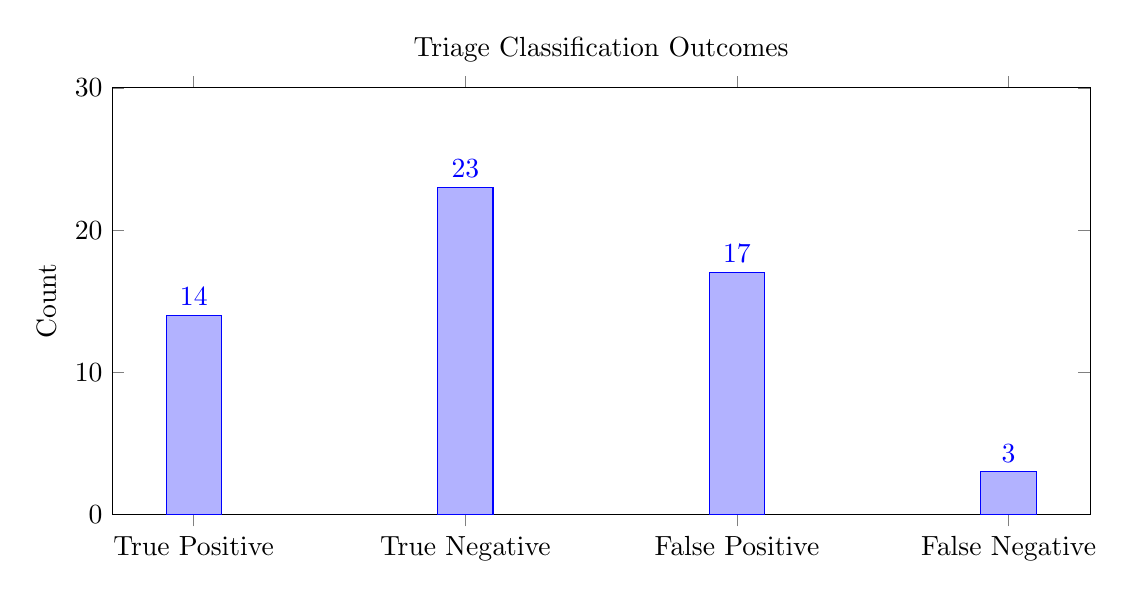
\begin{tikzpicture}
\begin{axis}[
    ybar,
    ymin=0,
    ymax=30,
    bar width=20pt,
    width=14cm,
    height=7cm,
    ylabel={Count},
    symbolic x coords={TP,TN,FP,FN},
    xticklabels={
        {True~Positive},
        {True~Negative},
        {False~Positive},
        {False~Negative}
    },
    xtick=data,
    nodes near coords,
    nodes near coords align={vertical},
    title={Triage Classification Outcomes},
]
\addplot coordinates {(TP,14) (TN,23) (FP,17) (FN,3)};
\end{axis}
\end{tikzpicture}
\caption{Distribution of classification outcomes across the dataset.}
\label{fig:classification_outcomes}
\end{figure}


The bar chart in Figure~\ref{fig:classification_outcomes} summarises how the system classified the 134 crash instances in the dataset.  
Most predictions fall into the True Negative (23) and False Positive (17) categories, indicating that the model frequently flagged benign crashes as vulnerabilities.  
Conversely, the system correctly identified 14 genuine vulnerabilities (True Positives) and missed only 3 (False Negatives).  
This distribution suggests that the model favours recall—successfully detecting most real vulnerabilities—but at the cost of a higher number of false alarms.

\begin{table}[ht]
\centering
\begin{tabular}{|l|c|}
\hline
\textbf{Metric} & \textbf{Value} \\
\hline
\hline
Accuracy  & 0.6491 \\
Precision & 0.4516 \\
Recall    & 0.8235 \\
F1 Score  & 0.2917 \\
\hline
\end{tabular}
\caption{Evaluation metrics computed from the classification results.}
\label{tab:eval_metrics}
\end{table}



Table~\ref{tab:eval_metrics} reports the derived performance metrics.  
The overall accuracy (0.6491) reflects the proportion of correct classifications across all crashes, though it is influenced by the imbalance between benign and vulnerable samples.  
Precision (0.4516) is relatively low, consistent with the high number of False Positives observed in the chart; many issues flagged as vulnerabilities did not correspond to real security risks.  
Recall (0.8235) is considerably higher, showing that the system is effective at capturing genuine vulnerabilities and rarely overlooks dangerous cases.  
However, the F1-score (0.2917)—the harmonic mean of precision and recall—is low, indicating an uneven balance between detecting vulnerabilities and avoiding false alarms.

Overall, these results show that the current implementation is conservative in its judgement, prioritising the detection of potential vulnerabilities over strict precision.  
While this behaviour is desirable in contexts where missing a vulnerability is more costly than over-reporting, it also highlights the need for improvements aimed at reducing false positives, such as integrating specialised models, adopting RAG-based grounding, or leveraging persistent agents as discussed in Chapter~\ref{chp:futureWork}.

    \chapter{Discussion}
\label{chp:disc}

\section{Tool Performance and Efficiency}

The implemented pipeline demonstrates acceptable and promising operational performance.  


\textit{Single-crash} analysis by the \gls{llm} requires on average less than a minute, which makes the approach scalable and significantly accelerates the classification process.
However, the total execution time per application depends heavily on fuzzing procedure, the crash count of method, the complexity of native stack traces, and the number of native libraries involved.  
In applications with many or large native libraries, the overhead caused by importing and decompiling binaries can substantially increase the total runtime, this overhead originates from the reverse-engineering tools rather than from the analysis performed by the model.

\section{Effect of \glsxtrlong{jcg}}

As seen in Chapter~\ref{chp:result}, the comparison between analyses performed with or without the \gls{jcg} yields a clear trade-off:

\begin{myitemize}
    \item When the \glsxtrlong{jcg} is available (“With \glsxtrshort{jcg}”), the model can leverage both native and Java-level context, producing more coherent and realistic vulnerability assessments. Under this configuration, the system achieves higher recall and maintains relatively few false negatives.
    \item Without the \glsxtrlong{jcg} (“Without \glsxtrshort{jcg}”), the lack of Java-side context leads the model to over-approximate risks. Without knowing the origin or constraints of the data, the system tends to treat values as attacker-controlled, even when in reality they may originate from fixed Java-side logic and be impossible for an attacker to influence.
\end{myitemize}




\section{Reliability}

The pipeline exhibits a low number of False Negatives, indicating that genuine vulnerabilities are rarely overlooked. This behaviour is partly influenced by the \gls{llm}'s tendency to classify ambiguous memory-related faults (e.g., buffer errors, JNI misuse, invalid native calls) as potentially dangerous. Prior studies highlight similar patterns: general-purpose models often over-predict positives, hallucinate tool behaviour, or misinterpret control-flow semantics~\cite{10456393,ullah2024llmsreliablyidentifyreason}. 

\section{Limitations}

The evaluation performed in this thesis is subject to several limitations that affect the results.

The quality of the classification strongly depends entirely on the crash traces produced by POIROT. When stack trace contain missing or unresolved entries (marked as ``\texttt{??}''), the model lacks essential execution context and tends to assume a worst-case scenario, contributing to the high false-positive rate observed in the evaluation.

The dataset, though representative of diverse applications, cannot fully capture the variability of real-world Android ecosystems. 



%-------------------------------------------------------------------------
%-------------------------------------------------------------------------
%-------------------------------------------------------------------------
%-------------------------------------------------------------------------



\section{Comparison with Ground-Truth Vulnerability}
\label{sec:comparison_tpcamera}

To evaluate the quality of the \gls{llm}-based triage, this section compares the model’s classification of a real vulnerability in the \texttt{tpCamera} application with the ground truth reported in the POIROT paper~\cite{poirot-usenix25}.  
The vulnerability, later assigned CVE-2023-30273, concerns a use-after-free condition in the native MP4 encoding library.

\subsection{Ground-Truth Summary}
Section~5.6 of the POIROT paper describes a reproducible use-after-free vulnerability in the \texttt{libTPMp4Encoder.so} library.  
The flaw arises when the application invokes the MP4 encoding pipeline with malformed JPEG or H.264 data:

\begin{itemize}
    \item The JNI function \texttt{packVideo} receives attacker-controlled frame data and a size parameter.
    \item The native function \texttt{mp4\_write\_one\_h264} tears down the encoder context on malformed input: it closes the file, frees multiple internal buffers, and finally frees the global structure \texttt{iniPacker\_global} itself.
    \item A second invocation of \texttt{packVideo} reuses the same freed encoder context, triggering a \emph{use-after-free} where the freed structure is overwritten by attacker-controlled data.
    \item The overwritten structure corrupts the file pointer passed to \texttt{fclose()}, enabling arbitrary code execution under certain conditions.
\end{itemize}

The exploit is reproducible with a precise call sequence (\texttt{iniPacker} → \texttt{packVideo} → second \texttt{packVideo}) and was validated both locally and through a MITM attack against the tpCamera app.

\subsection{LLM Classification Summary}
\ref{out}

The \gls{llm}-based triage correctly identifies the crash in \texttt{tpCamera} as a genuine vulnerability, assigning a high severity level and a confidence score of 0.85.  
The model attributes the crash to a memory-safety error in the native MP4 encoding pipeline, centred around the logic implemented in the \texttt{mp4\_write\_one\_h264} routine in \texttt{libTPMp4Encoder.so}.

The full classification output for this application is provided in Appendix~\ref{chp:appendixA}.

\medskip

\noindent The classification highlights three main contributing factors:

\begin{itemize}
    \item \textbf{Unvalidated size parameter}: The JNI method \texttt{packVideo} forwards an unbounded, attacker-influenced size directly to the native encoder without consistency checks.
    
    \item \textbf{Unsafe error-handling path}: On malformed Network Abstraction Layer (NAL) input, \texttt{mp4\_write\_one\_h264} frees multiple internal buffers and then frees the encoder context itself, while higher-level code may continue using the same structure.

    \item \textbf{Potential heap corruption and double free}: Repeated calls on a freed context can corrupt heap metadata, consistent with the crash \texttt{scudo::reportInvalidChunkState}.
\end{itemize}

The model concludes that the vulnerability likely enables heap corruption or a double-free/use-after-free condition, mapping it to CWE-787 (Out-of-bounds Write), CWE-415 (Double Free), and CWE-416 (Use After Free).  
It also identifies a plausible exploitation vector: \texttt{"trigger\_method"}: ``Malformed H.264 frame buffer passed via MP4Encoder.packVideo with inconsistent size parameter''.

\subsection{Comparison with Ground Truth}

The \gls{llm}-generated analysis aligns closely with the ground-truth description reported in the POIROT paper~\cite{poirot-usenix25}.  
Both sources identify the vulnerability as a use-after-free condition arising from repeated invocations of \texttt{packVideo} on a freed encoder context.

\paragraph{\glsxtrlong{llm} classification compared with PIROT}

\begin{itemize}
    \item \textbf{Root cause agreement}: The analysis matches the PIROT description, recognising that the encoder context (\texttt{iniPacker\_global}) is freed on malformed input and later reused, enabling a use-after-free.
    \item \textbf{Impact on file handling}: The classification highlights that tearing down and reusing the encoder context affects file and stream management, which is consistent with the PIROT finding that corruption of this context can influence the \texttt{FILE*} pointer passed to \texttt{fclose()}.
    \item \textbf{Attack preconditions}: It correctly notes that the vulnerability is remotely triggerable through malformed video frames delivered over an untrusted network channel.
    \item \textbf{Code execution potential}: The analysis further infers that this memory-safety primitive can lead to arbitrary function invocation or code execution under realistic conditions.
\end{itemize}

Overall, the model captures the key structural and behavioural elements of the vulnerability, providing an analysis that is consistent with the real exploit chain reported in the ground-truth study.

\subsection{Interpretation of Results}

This comparison shows that the \gls{llm}-based triage is capable of reconstructing the essential characteristics of a complex native vulnerability using only stack-trace evidence, decompiled code, and contextual information accessed through \gls{mcp} tools.  
The model correctly identifies the use-after-free pattern, the conditions that lead to encoder-state corruption, and the attacker-controlled inputs required to reach the vulnerable code paths.

The analysis produced by the model is not only consistent with the POIROT ground truth, but also captures several realistic exploitation vectors.  
Its focus on the unvalidated size parameter, while not explicitly central in the POIROT paper, illustrates the model's ability to reason about alternative failure modes that could plausibly contribute to heap corruption in similar contexts.

The case study demonstrates that the proposed pipeline can approximate expert-level reasoning and align closely with real-world vulnerability reports, validating its effectiveness as an initial triage mechanism.


    \chapter{Conclusions}
\label{chp:conclusions}

This thesis presented an automated triage pipeline that combines Large Language Models with the Model Context Protocol (MCP) to analyse native crashes in Android applications.  
The goal was to support vulnerability assessment in settings where manual crash inspection is costly, and where modern applications integrate substantial amounts of native code exposed through the Java Native Interface.

The proposed system integrates reverse-engineering tools---Jadx for bytecode analysis and Ghidra for native disassembly---into the LLM’s reasoning loop, enabling context-aware classification of POIROT-generated crashes.  
The evaluation demonstrates that the pipeline reliably identifies real vulnerabilities, achieving consistently low false-negative rates and providing structured explanations, confidence scores, and evidence traces.  
The tpCamera case study further shows that the system can approximate expert-level analysis: the LLM classification aligns with the ground-truth vulnerability reported in PIROT (CVE-2023-30273), correctly identifying the unsafe lifecycle of the encoder context and the conditions leading to a use-after-free.

At the same time, the results highlight several limitations.  
Precision remains modest, primarily due to incomplete crash traces and the conservative behaviour of general-purpose LLMs, which tend to over-approximate risk when information is missing.  
Additional restrictions arise from partial decompilation, the heterogeneity of Android JNI patterns, and the uncertainty inherent to LLM-based reasoning.  
These findings indicate that such a system should not replace traditional analyses, but rather act as an initial filter that accelerates and prioritises manual investigation.

Despite these limitations, the work demonstrates the viability of using LLMs to enhance automated vulnerability triage.  
The approach scales to applications with numerous native libraries, reduces the manual burden on analysts, and provides reproducible reasoning grounded in explicit code evidence.  
This opens opportunities for integrating LLM-assisted triage into broader fuzzing pipelines or continuous security testing frameworks.

Future work should focus on improving precision through richer static and dynamic context, extending Java–to–native call-graph reconstruction, and exploring ensemble or multi-agent architectures to reduce uncertainty.  
Integrating automated exploitability assessment and symbolic reasoning layers could also further strengthen the system’s reliability.  

In conclusion, this thesis shows that LLM-based crash triage, when combined with reverse-engineering tools through MCP, offers a promising direction for scalable vulnerability analysis.  
It enhances the efficiency and consistency of the triage process and provides a practical foundation for more advanced, context-aware security automation.


    % \include{chapters/dataset}
    % \include{chapters/models}
    % \include{chapters/results}
    % \include{chapters/conclusion}
    
    % afterword
    \cleardoublepage
    \phantomsection
    \addcontentsline{toc}{chapter}{References}
    \bibliography{references.bib}
    
    \cleardoublepage
    \phantomsection
    \addcontentsline{toc}{chapter}{Acknowledgments}
    \acknowledgments

\end{document}